%\documentclass[BTech]{iiitdmdiss}
%\documentclass[DD]{iiitdmdiss}
\documentclass[BTech]{iiitdmdiss}
\usepackage{times}
\usepackage{tikz}
\usepackage{t1enc}
\usepackage[utf8]{inputenc}
\usepackage{multicol}
\usepackage{multirow}
\usepackage{placeins}
\usepackage{pgfplots}
\usepackage{graphicx}
\usepackage{booktabs}
\usepackage{longtable}
\usepackage{array}
\usepackage{xcolor}
\usepackage{colortbl}
\usepackage{booktabs}
\usepackage{longtable}
\usepackage{array}
\usepackage{graphicx}
\usepackage{subcaption}
\usepackage{xcolor}
\usepackage{colortbl}
\usepackage{pgfplots}
\pgfplotsset{compat=1.18}
\usepackage{epstopdf}
\usepackage{fancyhdr}
\setlength{\headheight}{14.5pt} % make headheight big enough for fancyhdr
\usepackage[driverfallback=dvipdfm]{hyperref} % hyperlinks for references.
\usepackage{amsmath} % easier math formulae, align, subequations \ldots
\renewcommand{\headrulewidth}{1pt}
\renewcommand{\footrulewidth}{1pt}

% --- Encoding & Font ---
\usepackage[utf8]{inputenc}
\usepackage[T1]{fontenc}

% --- Page Layout ---
\usepackage{geometry}
\geometry{margin=2.5cm}

% --- Math ---
\usepackage{amsmath, amssymb}
\usepackage{mathtools}

% --- Graphics & Figures ---
\usepackage{graphicx}
\usepackage{caption}
\usepackage{subcaption}

% --- Tables ---
\usepackage{booktabs}

% --- Lists ---
\usepackage{enumitem}

% --- Hyperlinks ---
\usepackage{hyperref}
\hypersetup{
    colorlinks=true,
    linkcolor=blue,
    citecolor=blue,
    urlcolor=blue
}

% --- Algorithms ---
\usepackage{algorithm}
\usepackage{algpseudocode}

% --- Code Listings (critical for chapter 3) ---
\usepackage{listings}
\usepackage{xcolor}

\lstdefinestyle{pythonstyle}{
    backgroundcolor=\color{gray!10},
    commentstyle=\color{green!60!black},
    keywordstyle=\color{blue},
    numberstyle=\tiny\color{gray},
    stringstyle=\color{orange},
    basicstyle=\ttfamily\footnotesize,
    breakatwhitespace=false,
    breaklines=true,
    captionpos=b,
    keepspaces=true,
    numbers=left,
    numbersep=5pt,
    showspaces=false,
    showstringspaces=false,
    showtabs=false,
    tabsize=2,
    language=Python
}


\begin{document}


%%%%%%%%%%%%%%%%%%%%%%%%%%%%%%%%%%%%%%%%%%%%%%%%%%%%%%%%%%%%%%%%%%%%%%
% Title page
%-----------------------------------------------
% Provide all the necessary information here
%-----------------------------------------------
\title{Multimodal Optimal Transport Self-Supervised Learning for Unified Chest X-ray Classification, Localization, and Automated Report Generation}
\author{Aditya Pillai}
\roll{CS22B1063}
\monthyear{May 2026}
\department{Computer Science and Engineering}
\guide{Dr. Umarani Jayaraman}
\guidedesignation{Assistant Professor}
\guidedept{Computer Science and Engineering}
\date{11.05.2026}

\nocite{*} % include all bibliography entries even if not cited
\maketitle

%%%%%%%%%%%%%%%%%%%%%%%%%%%%%%%%%%%%%%%%%%%%%%%%%%%%%%%%%%%%%%%%%%%%%%
% Declaration of originality
\declaration

%%%%%%%%%%%%%%%%%%%%%%%%%%%%%%%%%%%%%%%%%%%%%%%%%%%%%%%%%%%%%%%%%%%%%%

% Certificate
\certificate
%%%%%%%%%%%%%%%%%%%%%%%%%%%%%%%%%%%%%%%%%%%%%%%%%%%%%%%%%%%%%%%%%%%%%%
% Acknowledgements
\acknowledgements

I would like to take this opportunity to express my gratitude to my advisor, Dr. Umarani Jayaraman , whose guidance, expertise, and support have very helpful throughout this research journey. Her insightful feedback and constructive criticism have immensely enriched the quality of this project. I would like to acknowledge the contributions of my peers who have provided insightful discussions and feedback during the course of this research project. Your input has been invaluable in shaping the direction and scope of this paper. I am grateful to all the faculty members of IIITDM Kancheepuram, who have given me the foundational knowledge in the field of computer science with their insightful lectures, mentorship, and guidance.

%%%%%%%%%%%%%%%%%%%%%%%%%%%%%%%%%%%%%%%%%%%%%%%%%%%%%%%%%%%%%%%%%%%%%%
% Abstract
\abstract
Chest X-ray interpretation is an essential diagnostic task that faces the issues of radiologist scarcity, label noise, and class imbalance in large-scale datasets. In this paper, an OPTiML-inspired self-supervised learning pipeline is proposed for multi-label thoracic disease classification on the NIH ChestX-ray14 dataset. In the proposed approach, a dense EfficientNet-B3 backbone is first pretrained without any disease labels using a composite loss that combines Sinkhorn optimal transport alignment, variance regularisation, and covariance decorrelation. Then, the pretrained EfficientNet-B3 backbone is fine-tuned in a multimodal supervised learning approach that incorporates image features with patient metadata including age, gender, and view position. The proposed approach attains a mean AUC-ROC of 0.8636 across 13 disease classes, outperforming the performance of several strong baselines including DenseNet-121 (0.77), ViT/Swin (0.80), and EfficientNet-B3 without SSL pretraining (0.85). Moreover, the proposed approach attains an improvement in Macro F1 from 0.3444 to 0.5103 using per-class threshold optimisation by calibrating the decision boundaries below 0.5, which were completely suppressed by the default threshold. Additional tasks verify the spatial quality of the learned representations, including lung segmentation with a Dice coefficient of 0.9537 and bounding box localisation with an IoU of 0.22 using weak supervision. At the end a radiology report is also created using the generated bounding boxes and the predicted labels. Overall, the results demonstrate that OPTiML-inspired self-supervised pretraining is an effective strategy for medical image analysis, particularly in scenarios with noisy or imbalanced labels, and validates the feasibility of the proposed pipeline inspired by the original OPTiML paper.
\\
\vspace{10pt}
\noindent KEYWORDS: \hspace*{0.5em} \parbox[t]{4.4in}{Self-Supervised Learning; Optimal Transport; Multi-Label Classification; Chest X-Ray; EfficientNet-B3; Focal Loss.}

%%%%%%%%%%%%%%%%%%%%%%%%%%%%%%%%%%%%%%%%%%%%%%%%%%%%%%%%%%%%%%%%%
% Table of contents etc.

\begin{singlespace}
\tableofcontents
\thispagestyle{empty}

\listoftables
\addcontentsline{toc}{chapter}{LIST OF TABLES}
\listoffigures
\addcontentsline{toc}{chapter}{LIST OF FIGURES}
\end{singlespace}


%%%%%%%%%%%%%%%%%%%%%%%%%%%%%%%%%%%%%%%%%%%%%%%%%%%%%%%%%%%%%%%%%%%%%%
% Abbreviations
% \abbreviations

% \noindent 
% \begin{tabbing}
% xxxxxxxxxxx \= xxxxxxxxxxxxxxxxxxxxxxxxxxxxxxxxxxxxxxxxxxxxxxxx \kill
% \textbf{DSP}   \> Digital Signal Processing\\

% \end{tabbing}
\abbreviations
\noindent
\begin{tabbing}
xxxxxxxxxxxx \= xxxxxxxxxxxxxxxxxxxxxxxxxxxxxxxxxxxxxxxxxxxxxxxxxxxxxxxx \kill
\textbf{AP}         \> Anteroposterior\\
\textbf{AUC}        \> Area Under the Curve\\
\textbf{AUC-ROC}    \> Area Under the Receiver Operating Characteristic Curve\\
\textbf{CAD}        \> Computer-Aided Diagnosis\\
\textbf{CXR}        \> Chest X-Ray\\
\textbf{F1}         \> F1 Score (Harmonic Mean of Precision and Recall)\\
\textbf{Grad-CAM}   \> Gradient-weighted Class Activation Mapping\\
\textbf{HiTL}       \> Human in the Loop\\
\textbf{IHRAS}      \> Intelligent Humanized Radiology Analysis System\\
\textbf{IoU}        \> Intersection over Union\\
\textbf{KL}         \> Kullback--Leibler Divergence\\
\textbf{MBConv}     \> Mobile Inverted Bottleneck Convolution\\
\textbf{MIMIC-CXR}  \> Medical Information Mart for Intensive Care -- Chest X-Ray\\
\textbf{NIH}        \> National Institutes of Health\\
\textbf{OPTiML}     \> Optimal Transport Inspired Machine Learning\\
\textbf{OT}         \> Optimal Transport\\
\textbf{PA}         \> Posteroanterior\\
\textbf{RAG}        \> Retrieval-Augmented Generation\\
\textbf{ReLU}       \> Rectified Linear Unit\\
\textbf{ROC}        \> Receiver Operating Characteristic\\
\textbf{SE}         \> Squeeze-and-Excitation\\
\textbf{SimCLR}     \> Simple Framework for Contrastive Learning of Visual Representations\\
\textbf{SOTA}       \> State of the Art\\
\textbf{SSL}        \> Self-Supervised Learning\\
\textbf{t-SNE}      \> t-distributed Stochastic Neighbour Embedding\\
\textbf{ViT}        \> Vision Transformer\\
\end{tabbing}


\notation
\noindent
\begin{tabbing}
xxxxxxxxxxxxxxxxxxxxxxxxxxxxxxxxxx \= xxxxxxxxxxxxxxxxxxxxxxxxxxxxxxxxxxxxxxxxxxxxxxx \kill

\textbf{Symbol} \> \textbf{Description}\\[0.4em]

$X \in \mathbb{R}^{H \times W \times 3}$    \> Input chest X-ray image\\
$Y \in \{0,1\}^{C}$                         \> Ground-truth multi-hot label vector\\
$\hat{Y} \in [0,1]^{C}$                     \> Predicted disease probability vector\\
$C$                                          \> Number of disease classes\\
$f(\cdot)$                                   \> Encoder backbone (EfficientNet-B3)\\
$g(\cdot)$                                   \> Projection head (SSL stage)\\
$\mathbf{z}_{img}$                           \> Image feature vector, $\in \mathbb{R}^{1536}$\\
$\mathbf{z}_{meta}$                          \> Metadata feature vector, $\in \mathbb{R}^{16}$\\
$\mathbf{z}_1,\, \mathbf{z}_2$              \> Patch-level SSL embeddings, $\in \mathbb{R}^{B \times HW \times D}$\\
$\mathbf{C},\, \mathbf{T}$                  \> OT cost matrix and transport plan\\
$\mathcal{L}_{\text{SSL}}$                   \> Total SSL loss\\
$\mathcal{L}_{\text{OT}},\, \mathcal{L}_{\text{var}},\, \mathcal{L}_{\text{cov}}$ \> OT alignment, variance, covariance losses\\
$\lambda_{\text{var}} = 0.1,\; \lambda_{\text{cov}} = 0.01$ \> SSL loss weights\\
$\mathcal{L}_{\text{Focal}}$                 \> Multi-label Focal Loss\\
$\alpha = 0.25,\; \gamma = 2.0$             \> Focal loss parameters\\
$\tau_c$                                     \> Per-class decision threshold\\
$\eta$                                       \> Learning rate\\
$\mu,\, \sigma$                              \> ImageNet normalisation mean and std\\

\end{tabbing}

\pagebreak
\clearpage

% The main text will follow from this point so set the page numbering
% to arabic from here on.
\pagenumbering{arabic}
\pagestyle{fancy}
\fancyhf{}

%%%%%%%%%%%%%%%%%%%%%%%%%%%%%%%%%%%%%%%%%%%%%%%%%%%
%Enter the details of roll number, department and year for Header and Footer
%%%%%%%%%%%%%%%%%%%%%%%%%%%%%%%%%%%%%%%%%%%%%%%%%%%
\fancyhead[l]{\leftmark}
\fancyfoot[r]{\thepage}
\fancyhead[r]{CS22B1063}
\fancyfoot[l]{Department of CSE, IIITDM Kancheepuram, May 2026}

%%%%%%%%%%%%%%%%%%%%%%%%%%%%%%%%%%%%%%%%%%%%%%%%%%
\chapter{INTRODUCTION}
\graphicspath{{Chapter1/}}

\section{Background}
Chest X-ray or chest radiography has been for a long time a widely used and cost-effective imaging technique for the diagnosis and monitoring of thoracic diseases, which include diseases like pneumonia, TB, edema, lung nodules, etc. The major reasons behind this are the accessibility, low radiation exposure (so low risk), and non-invasive nature of this technique. However, the study of these radiographs requires expertise, and the growing volume of imaging studies has created a demand that is difficult to meet considering the limited availability of trained radiologists; therefore, there is a need for automated and computer-aided diagnostic (CAD) systems.
\newline
Although recent advancements in AI, specifically Deep Learning, have achieved significant success in medical image analysis, to be more precise, Convolutional Neural Networks (CNNs) and recent Vision Transformer (ViT) models have achieved promising performance in disease classification, abnormality detection, and segmentation. Despite these advancements, several problems and challenges still remain, such as relying heavily on supervised learning, i.e., large volumes of labeled data. Another problem is that many such models operate as black boxes, i.e., interpretability is too low pertaining to the spatial grounding and extent of abnormalities, and in clinical settings, interpretability is important and highly appreciated.


\section{Problem Statement}

Although deep learning models have achieved promising results in multi label chest X-ray classification, most existing systems:

\begin{itemize}
    \item Operate as black-box classifiers.
    \item Do not provide spatial localization of detected pathologies.
    \item Do not generate clinically structured radiology reports.
    \item Lack explainability and fine-grained disease-region alignment.
\end{itemize}

There is therefore a need for an end-to-end, explainable, and multimodal AI system that can:

\begin{enumerate}
    \item Learn robust visual representations from large-scale chest X-ray data.
    \item Perform multi label disease classification.
    \item Localize pathological regions.
    \item Provide interpretable evidence for predictions.
    \item Generate structured radiology-style reports.
\end{enumerate}

\section{Formal Problem Definition}

\subsection{Input}

For each patient case, the system receives:

\begin{enumerate}
    \item A chest X-ray image:
\[
X \in \mathbb{R}^{H \times W \times 3}
\]

\begin{figure}[H]
    \centering
    
    % --- Three X-rays in a single row ---
    \begin{subfigure}{0.32\textwidth}
        \centering
        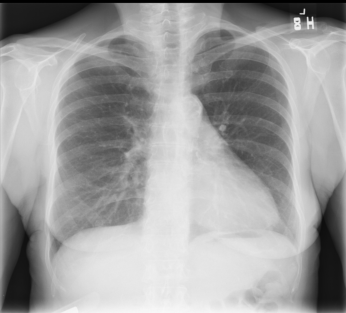
\includegraphics[width=\linewidth,height=0.18\textheight,keepaspectratio]{xray1.png}
        \caption{Sample X-ray 1}
    \end{subfigure}
    \hfill
    \begin{subfigure}{0.32\textwidth}
        \centering
        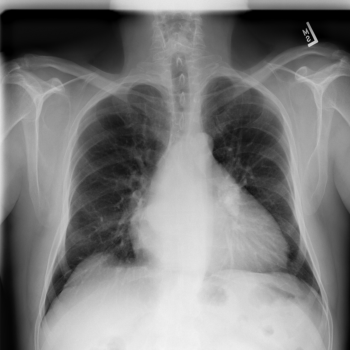
\includegraphics[width=\linewidth,height=0.18\textheight,keepaspectratio]{xray2.png}
        \caption{Sample X-ray 2}
    \end{subfigure}
    \hfill
    \begin{subfigure}{0.32\textwidth}
        \centering
        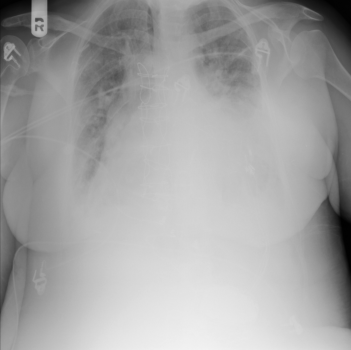
\includegraphics[width=\linewidth,height=0.18\textheight,keepaspectratio]{xray3.png}
        \caption{Sample X-ray 3}
    \end{subfigure}

    \vspace{0.3cm}

    % --- Metadata dataframe image below ---
    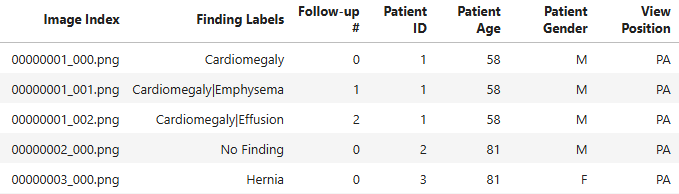
\includegraphics[width=0.8\textwidth,height=0.25\textheight,keepaspectratio]{metadata_dataframe.png}
    
    \caption{Example chest X-ray samples (top) and corresponding patient metadata (bottom).}
    \label{fig:input_samples}
\end{figure}
    \item Patient metadata:
    \[
    M = \{\text{Age}, \text{Gender}, \text{View Position}\}
    \]

    \item (During training) Ground-truth multi-label disease annotations:
    \[
    Y \in \{0,1\}^{C}
    \]
    where \( C \) denotes the number of disease classes.

    \item (Optionally during training) Bounding box annotations for disease localization.

    \item (Optionally during training) Corresponding radiology reports for text generation.
\end{enumerate}
\subsection{Output}

The system is required to produce:

\begin{enumerate}
    \item Multi-label disease prediction probabilities:
    \[
    \hat{Y} \in [0,1]^{C}
    \]

    \item Binary disease decisions after thresholding:
    \[
    \tilde{Y} \in \{0,1\}^{C}
    \]

    \item Predicted bounding boxes
    Let the input image be defined as:

\[
X \in \mathbb{R}^{H \times W \times 3}
\]

where \(H\) and \(W\) denote the height and width of the image.

For each disease class \(c \in \{1, 2, \dots, C\}\), the model predicts at most one bounding box corresponding to the detected pathological region.

The predicted bounding box for class \(c\) is defined as:

\[
\hat{b}_c = \left( x_c^{(1)}, y_c^{(1)}, x_c^{(2)}, y_c^{(2)} \right)
\]

such that:

\[
0 \leq x_c^{(1)} < x_c^{(2)} \leq W
\]

\[
0 \leq y_c^{(1)} < y_c^{(2)} \leq H
\]

where:

\begin{itemize}
    \item \( (x_c^{(1)}, y_c^{(1)}) \) denotes the top-left corner,
    \item \( (x_c^{(2)}, y_c^{(2)}) \) denotes the bottom-right corner,
    \item Coordinates are expressed in the same spatial reference frame as the input image.
\end{itemize}

    
    \item A structured radiology report:
    \[
    \hat{R} = \text{Generated textual report describing findings and impressions}
    \]
\end{enumerate}

\section{Motivation}

The global healthcare system continues to face an increasing burden of pulmonary diseases such as pneumonia, pneumothorax, edema, etc. Among the widely used cost-effective diagnostic tools for detecting such problems and diseases is the chest X-ray (CXR). Hospitals generate thousands of chest radiographs daily, especially at tertiary centers and emergency departments. But again, the issue is that accurate interpretation of these images requires trained radiologists, so in situations where human resources are scarce, backlogs are created. This leads to late diagnosis, which may even prove fatal, so obviously there is a need for rapid and reliable chest X-ray interpretation.

The primary motivation for pursuing this project is to develop a unified, explainable chest X-ray analysis system that leverages the abilities of SSL (Self-Supervised Learning), multi-label classification, bounding box localization, and automated report generation to bridge the gap between simple image-level prediction and clinically useful results.

Another key motivation is the need to address the limitations of supervised learning in medical imaging systems. Labeled datasets suffer from issues of class imbalance and a scarcity of abnormalities in the dataset, which makes it difficult to train a model to learn useful features.

There has also been a growing need to produce AI models in medical and healthcare systems, especially ones that have interpretability and can ground predictions spatially. This is because having explainability in a system allows the HiTL (Human in the Loop) to check if the predictions are right and whether the reason for those predictions is also right. This also helps in training a model based on feedback (Reinforcement Learning).

\section{Objectives}
\subsection{Primary Objectives}
The primary objective of this project is to enhance the classification capability and performance on chest X-rays using advanced representational learning and optimization strategies.
\begin{enumerate}
\item The objective is to improve the classification performance (AUC and F1 are the metrics of concern) using architectures like EfficientNet or Vision Transformers (like Swin and DINO).
\item To integrate SSL (Self-Supervised Learning) as a pretraining step before supervised learning so that the model can learn robust anatomical features from unlabeled data.
\item To study the impact of introducing SSL compared to just using common deep learning models for better generalization ability.
\item To analyze the model's robustness by calculating per-class AUC and macro/micro F1 scores.
\item To compare various architectures like EfficientNet, DenseNet, and Swin/DINO to determine the best feature extractor for the task.
\end{enumerate}
\subsection{Secondary Objectives}
The secondary objective is to design an end-to-end pipeline that extends beyond just classification to a complete chest radiology system.

\begin{enumerate}
\item To implement bounding box localization of diseases; this ensures spatial grounding.
\item To perform segmentation of the lung region to identify regions within the lungs for radiology report generation and spatial grounding.
\item To develop a radiology report generation module that can use structured outputs to generate logical and relevant textual reports.
\end{enumerate}

\subsection{Tertiary Objectives}
To design a complete GUI and backend framework and deploy the solution for public usage with necessary caution, permissions, and licenses.
\chapter{Literature Survey}
\graphicspath{{Chapter2/}}
The recent developments in using deep learning models to automatically generate radiology reports for chest X-rays are the main topic of this review of the literature. It places special emphasis on clinical evaluation, explainability strategies, and multimodal models. From basic image captioning, the field has developed into complex models that integrate clinical reasoning, knowledge representation, and image understanding. Anatomical attention mechanisms, retrieval-augmented generation, vision-language alignment, and explainability concept bottleneck models are some of the important topics that have been investigated. The goal of this review is to identify research gaps that require attention, such as correcting hallucinations, quantitatively validating explainability, and adding structured clinical context, as well as to highlight the SOTA work currently in use and evaluate their strengths and weaknesses.
\section{Multimodal Learning Architectures}
This technique tries to jointly model visual and textual findings for automated chest x-ray report generation, this is not just simple image captioning, these architectures try to capture by linking image features with medical terminologies.
\subsection{Knowledge-Enhanced Report Generation}
This approached was put forward by Yang et al. and it introduces a medical knowledge base that is learned during training. Instead of relying on predefined medical knowledge and knowledge graphs the model learns semantic relationships between anatomical structures and clinical phrases.
The system aligns three modalities into a shared embedding space:
\begin{enumerate}
    \item Image features extracted from chest X-rays
    \item Textual representations of reports
    \item Disease label embeddings
\end{enumerate}
By enforcing alignment across these representations, the model learns how specific visual patterns correspond to specific medical concepts and language.
\subsubsection{Strengths}
Some of the strengths include
\begin{enumerate}
    \item Performance improvement in BLEU and ROUGE metrics in IU-XRAY and MIMIC-CXR datasets.
    \item Another major strength is reduction of manual engineering since this system avoids using manually created labels.
\end{enumerate}
\subsubsection{Weaknesses}
Some of the weaknesses are:
\begin{enumerate}
    \item There is a performance gain, that cannot be denied but the idea of a learned knowledge base lacks interpretability. Experts cannot directly tell what knowledge has been encoded.
    \item It does not provide region-level grounding nor pixel level.
\end{enumerate}

\subsection{Integration of Structured Clinical Context}
This goes beyond the previous knowledge base method as this extends and incorporates clinical information like:
\begin{enumerate}
    \item Vital Signs
    \item Symptoms
    \item Clinical Notes
    \item Patient History
\end{enumerate}
and it uses a cross headed multi attention mechanism to learn weights from different modalities while generating the report.
\subsubsection{Strengths}
Since we know that ML and DL are about mimicking human intelligence, this method come very close to it as radiologists rarely interpret X-rays in isolation. E.g. A patient comes with cough and cold then it obviously increases chance of lung infection.
\subsubsection{Weaknesses}
\begin{enumerate}
    \item A major problem that is not directly visible is confirmation bias, the model may overly rely on symptoms than actual structural/anatomical findings.
    \item Another key challenge is handling missing or inconsistent data so a model overly relying on structured data will become biased on absence of them.
\end{enumerate}
\subsection{Multi-Granularity Feature Fusion}
This method was proposed by Zhang et al. and relies on multi scale image feature extraction using Swin Transformers. These features will contain both global and local features.
This architecture uses:
\begin{enumerate}
    \item Multi Scale image features.
    \item Label Embeddings
    \item Patient History encoded with BioBERT
    \item A language decoder (DistilGPT2)
\end{enumerate}
\subsubsection{Strengths}
\begin{enumerate}
    \item Chest/Lung abnormalities occur at multiple scales. Large Pleural Effusions require global understanding whereas small masses and nodules require understanding at local level.
    \item This system proved better detector of subtle findings 
\end{enumerate}
\section{Modular and Component-Based Systems}
Unlike end to end modules, modular system decomposes report generation into interpretable stages.
\subsection{Clinical Pipeline Integration (IHRAS Framework)}
IHRAS or the Intelligent Humanized Radiology Analysis System by IHRAS Research Team implements such a pipeline which includes:
\begin{enumerate}
    \item Multi-label Disease Classification.
    \item Grad-CAM visualization.
    \item Anatomical segmentation.
    \item Structured language generation.
    
\end{enumerate}
\subsubsection{Strengths}
This modular design improves efficiency and is transparent. Each stage can be validated independently. Segmentation outputs provide anatomical grounding. Grad-CAM visualizations allow experts or radiologists to verify if the right regions were considered or not.
\subsubsection{Weaknesses}
Major drawback is cascading of bad results or errors across various stages as modules operated separately and error cannot propagate so final report quality may deteriorate.

\section{Retrieval-Augmented and Hybrid Approaches}
\subsection{Multimodal Retrieval-Based Generation}
This approach was given by Jeong et al. and as the name suggests relies on a large knowledge base (pre-training) to fetch historically similar cases for report generation.
\subsubsection{Strengths}
Retrieval anchors generation to real clinical examples, reducing hallucination. It improves factual consistency, especially for rare conditions.
\subsubsection{Limitations}
Performance depends heavily on retrieval accuracy. Novel cases that differ from historical data may be poorly handled.
It requires large curated datasets.
\subsection{Concept Bottleneck Models with RAG}
Approach by Chen and Wang integrate concept bottlenecks with multi-agent Retrieval-Augmented Generation.
The system first predicts explicit medical concepts (e.g., cardiomegaly, effusion). These interpretable concepts form a bottleneck. A retrieval system then gathers supporting evidence, and a coordinating agent generates the final report.
\subsubsection{Strengths}
\begin{enumerate}
    \item Concept vectors are human-interpretable. Experts can correct incorrect concepts before final generation.
    \item Hallucination is reduced because generation is guided by explicit concept detection and retrieved evidence.
    \item The architecture supports human-in-the-loop validation.

\end{enumerate}
\subsubsection{Weaknesses}
It increases system complexity and computational overhead. Concept prediction errors can still affect downstream retrieval and generation.
\section{Comparative Insight}
\begin{table}[h]
\centering
\caption{Comparitive Study of Literature Survey}
\label{tab:method_comparison}
\begin{tabular}{|p{4cm}|p{5.5cm}|p{5.5cm}|}
\hline
\textbf{Method} & \textbf{Strengths} & \textbf{Weaknesses} \\
\hline

Knowledge-Enhanced Report Generation 
& Performance improvement in BLEU and ROUGE metrics on IU-XRAY and MIMIC-CXR datasets. Reduces manual engineering since it avoids using manually created labels and predefined knowledge graphs. 
& Learned knowledge base lacks interpretability; experts cannot directly tell what knowledge has been encoded. Does not provide region-level grounding or pixel-level explanation. \\

\hline

Integration of Structured Clinical Context 
& Mimics human reasoning since radiologists rarely interpret X-rays in isolation. Incorporates vital signs, symptoms, clinical notes, and patient history to improve contextual decision-making. 
& Risk of confirmation bias where the model may overly rely on symptoms rather than structural/anatomical findings. Handling missing or inconsistent structured data is challenging and may introduce bias. \\

\hline

Multi-Granularity Feature Fusion 
& Captures abnormalities occurring at multiple scales. Global understanding helps detect large pleural effusions, while local features help detect small masses and nodules. Demonstrated better detection of subtle findings. 
& Increased architectural complexity due to multi-scale fusion and multiple components. May reduce interpretability because multiple feature levels are fused together. \\

\hline

Clinical Pipeline Integration (IHRAS Framework) 
& Modular design improves transparency and efficiency. Each stage (classification, Grad-CAM visualization, segmentation, structured generation) can be independently validated. Segmentation provides anatomical grounding and Grad-CAM enables expert verification of attended regions. 
& Cascading of errors across stages. Since modules operate separately, errors in early stages may deteriorate final report quality. \\

\hline

Multimodal Retrieval-Based Generation 
& Retrieval anchors generation to real clinical examples, reducing hallucination. Improves factual consistency, especially for rare conditions. 
& Highly dependent on retrieval accuracy. Novel cases different from historical data may be poorly handled. Requires large curated datasets. \\

\hline

Concept Bottleneck Models with RAG 
& Concept vectors are human-interpretable and allow expert correction before final generation. Reduces hallucination by guiding generation with explicit concept detection and retrieved evidence. Supports human-in-the-loop validation. 
& Increases system complexity and computational overhead. Concept prediction errors can affect downstream retrieval and generation. \\

\hline

\end{tabular}
\end{table}
% ================================================================
% Chapter 3: Proposed Approach and Methodology
% Included via \input{chapter3_methodology} in main.tex
% ================================================================
% Required packages (add these to main.tex if not already present):
%   \usepackage{amsmath, amssymb}
%   \usepackage{listings}
%   \usepackage{xcolor}
%   \usepackage{caption}
%   \usepackage{enumitem}
% ================================================================

\chapter{Proposed Approach and Methodology}
\label{chap:methodology}

\section*{Overview}

The primary work done as a part of this project is the development of an "OPTiML" inspired self supervised representation learning pipeline for chest X-ray analysis, followed by supervised multi label disease classification and downstream clinical tasks (which in this case is report generation).

Unlike traditional supervised pipelines, the proposed approach first learns structure aware radiographic representations that too \emph{without labels}, and then transfers these representations to improve disease classification performance.

The pipeline consists of four main stages:
\begin{enumerate}
    \item \textbf{OPTiML-inspired Self-Supervised Pretraining}
    \item \textbf{Supervised Multi-Label Classification}
    \item \textbf{Disease Localization \& Segmentation} 
    \item \textbf{Structured Radiology Report Generation}
\end{enumerate}


%------------------------------------------------------------------
\section{Dataset}
%------------------------------------------------------------------

\subsection{NIH ChestX-ray14}

The experiments for classification and disease localization are conducted on the NIH ChestX-ray14 dataset, one of the largest publicly available chest radiograph collections. The dataset is loaded from a structured CSV file containing image metadata and associated diagnostic labels.

The dataset has over 100,000 images (PA and AP of X-ray) of over 30K unique patients with the text-mined fourteen disease image labels (where each image can have multilabels), mined from the reports of those patients using NLP.

The dataset contains 14 thoracic disease categories annotated via natural language processing of radiology reports. After filtering labels with fewer than 1,000 positive cases to ensure statistical reliability, the final label set is mentioned further in the report (check results).

To address severe class imbalance, a stratified sampling strategy was used with a limit of \textbf{10,000 samples per class}, this ensures that one disease does not dominate the training.

\begin{lstlisting}[style=pythonstyle, caption={Stratified sampling with class cap}]
max_samples_per_class = 10000
counter = Counter()
selected_rows = []

for idx, row in df.iterrows():
    labels = row["Finding Labels"].split("|")
    if all(counter[l] >= max_samples_per_class
           for l in labels if l in ALL_LABELS):
        continue
    selected_rows.append(row)
    for l in labels:
        if l in ALL_LABELS:
            counter[l] += 1

df = pd.DataFrame(selected_rows)
\end{lstlisting}

For disease localization, the \textbf{NIH BBox\_List\_2017.csv} file provides expert-annotated pixel-coordinate bounding boxes for 880 images spanning 8 disease categories. Each row corresponds to a single (image, disease) pair with columns $(x, y, w, h)$ in absolute pixel coordinates relative to the original $1024 \times 1024$ image resolution. Metadata is joined from \texttt{Data\_Entry\_2017.csv} using the image filename as the key, with median-value defaults applied for any missing entries. The localization data is split 80/20 with stratification on disease label to preserve per-class representation.

\subsection{Shenzhen Chest X-ray}

Lung segmentation is trained on the \textbf{Shenzhen Chest X-ray dataset}, which contains frontal chest radiographs with corresponding expert-delineated binary lung masks. Training is restricted to \textbf{Normal} cases only (i.e., non-TB) to avoid confusing mask quality with pathology-related structural changes. An 85/15 train/validation split is used. Masks are matched to images by filename, with the mask filename being the image name suffixed by \texttt{\_mask}.


%------------------------------------------------------------------
\section{Preprocessing}
%------------------------------------------------------------------

All images are loaded as RGB using PIL and resized to a fixed resolution. Metadata features are patient age, gender, and X-ray view position which can be PA or AP are numerically encoded to serve as inputs to the multimodal classifier.

Multi-hot label encoding maps each comma-separated finding string to a binary vector of length equal to the number of disease classes:

\begin{lstlisting}[style=pythonstyle, caption={Multi-hot label encoding}]
def encode_labels(labels_str):
    target = np.zeros(len(ALL_LABELS), dtype=np.float32)
    for l in labels_str.split('|'):
        if l in ALL_LABELS:
            target[ALL_LABELS.index(l)] = 1.0
    return target
\end{lstlisting}

Optional Preprocessing is to keep only the PA views but different views can always be used.

Heavy Augmentation (Rare Classes)
This includes heavy transformations augmentation for rare classes so that the model can be more diverse.
Includes:
\begin{enumerate}
    \item Resize

    \item Random Horizontal Flip
    \item Random Rotation (±20°)
    \item Random Resized Crop (Zoom 0.8–1.0)
    \item Random Affine Translation (10%)
    \item Color Jitter (Brightness, Contrast, Saturation)
    \item ToTensor 
    \item Normalize

\end{enumerate}

For bounding box regression, all ground-truth boxes are converted from \emph{top-left corner form} $(x, y, w, h)$ to \emph{centre form} $(c_x, c_y, w, h)$ and normalized to $[0, 1]$ by dividing by the original image width and height:

\begin{equation}
c_x = \frac{x}{W} + \frac{w}{2W}, \quad c_y = \frac{y}{H} + \frac{h}{2H}, \quad \hat{w} = \frac{w}{W}, \quad \hat{h} = \frac{h}{H}
\end{equation}

Centre-form coordinates are easier to regress as the network learns offsets from a central point. All output coordinates are clamped to $[0,1]$ to prevent out-of-image predictions.

For segmentation, images are loaded as single-channel grayscale, resized to $512 \times 512$, and normalized with mean $0.5$ and standard deviation $0.5$. Lung masks are binarized at a pixel threshold of 127. Ground-truth edge maps are derived from the binary masks via morphological operations (dilation minus erosion using a $5 \times 5$ elliptical kernel).

%------------------------------------------------------------------
\section{Architecture}
%------------------------------------------------------------------

\subsection{Multimodal Supervised Classifier}

The supervised classification model is a \textbf{multimodal EfficientNet-B3} architecture that fuses image-derived features with structured patient metadata. The backbone is initialized from ImageNet pretrained weights and adapted for the chest X-ray domain. Below are the architecture summary diagram both top level summary followed by
a detailed layer-by-layer breakdown. The model consists of three main components: 
\begin{enumerate}
    \item \textbf{Image Branch} 
    \item \textbf{Metadata Branch}
    \item \textbf{Fusion Classifier Head}
\end{enumerate}
% ================================================================
% Architecture Table — MultiModalEfficientNetB3
% Include in main.tex preamble:
%   
%   
%   
%   
%   
% ================================================================

% ------------------------------------------------------------------
% TABLE 1: High-level architecture summary (recommended for report)
% ------------------------------------------------------------------
\begin{table}[ht]
\centering
\caption{High-level architecture of the MultiModal EfficientNet-B3 model.}
\label{tab:arch_highlevel}
\renewcommand{\arraystretch}{1.3}
\begin{tabular}{llccc}
\toprule
\textbf{Stage} & \textbf{Component} & \textbf{Output Shape} & \textbf{Params} \\
\midrule
\multicolumn{5}{l}{\textit{Image Branch EfficientNet-B3 Backbone (ImageNet pretrained)}} \\
\midrule
Stem        & Conv2d + BN + SiLU          & $B \times 40 \times 224 \times 224$   & 1,160  \\
Stage 1     & MBConv $\times$2            & $B \times 24 \times 224 \times 224$   & 2,178 \\
Stage 2     & MBConv $\times$3            & $B \times 32 \times 112 \times 112$   & 31,632 \\
Stage 3     & MBConv $\times$3            & $B \times 48 \times 56 \times 56$     & 76,632 \\
Stage 4     & MBConv $\times$5            & $B \times 96 \times 28 \times 28$     & 266,832\\
Stage 5     & MBConv $\times$5            & $B \times 136 \times 28 \times 28$    & 717,792 \\
Stage 6     & MBConv $\times$6            & $B \times 232 \times 14 \times 14$    & 2,430,060\\
Stage 7     & MBConv $\times$2            & $B \times 384 \times 14 \times 14$    & 2,614,800\\
Head        & Conv2d + BN + SiLU + AvgPool + Identity & $B \times 1536$        & 593,408 \\
\midrule
\multicolumn{5}{l}{\textit{Metadata Branch MLP}} \\
\midrule
FC + ReLU + Dropout & Linear(3 $\to$ 16) & $B \times 16$   & 64 \\
\midrule
\multicolumn{5}{l}{\textit{Fusion Classifier Head}} \\
\midrule
Concat      & $[\mathbf{z}_{img},\ \mathbf{z}_{meta}]$ & $B \times 1552$\\
FC + ReLU + Dropout & Linear(1552 $\to$ 512) & $B \times 512$ & 795,13 \\
Output      & Linear(512 $\to$ 14)    & $B \times 14$           & 7,182  \\
\midrule
\multicolumn{2}{l}{\textbf{Total Parameters}}       & & \textbf{$\sim$10.5M} & \\
\multicolumn{2}{l}{\textbf{Trainable (initial)}}    & & \textbf{$\sim$802K}  & \\
\multicolumn{2}{l}{\textbf{Trainable (after unfreeze)}} & & \textbf{$\sim$10.5M} & \\
\bottomrule
\end{tabular}
\end{table}


% ------------------------------------------------------------------
% TABLE 2: Detailed layer-by-layer summary (abridged per stage)
% ------------------------------------------------------------------
\FloatBarrier
\begin{longtable}{clcr}
\caption{Detailed layer-by-layer summary of the MultiModal EfficientNet-B3 backbone (abridged by stage).}
\label{tab:arch_detailed} \\
\toprule
\textbf{Layer \#} & \textbf{Layer Type} & \textbf{Output Shape} & \textbf{Param \#} \\
\midrule
\endfirsthead
\multicolumn{4}{c}{\tablename~\ref{tab:arch_detailed} (continued)} \\
\toprule
\textbf{Layer \#} & \textbf{Layer Type} & \textbf{Output Shape} & \textbf{Param \#} \\
\midrule
\endhead
\midrule
\multicolumn{4}{r}{\textit{Continued on next page}} \\
\endfoot
\bottomrule
\endlastfoot

% ---- Stem ----
\rowcolor{gray!15}
\multicolumn{4}{l}{\textbf{Stem}} \\
1  & Conv2d           & $[-1,\ 40,\ 224,\ 224]$ & 1,080 \\
2  & BatchNorm2d      & $[-1,\ 40,\ 224,\ 224]$ & 80    \\
3  & SiLU             & $[-1,\ 40,\ 224,\ 224]$ & 0     \\

% ---- Stage 1: MBConv x2 ----
\rowcolor{gray!15}
\multicolumn{4}{l}{\textbf{Stage 1 MBConv $\times$2 (Squeeze-Excitation)}} \\
4--15  & Conv2d / BN / SiLU / SqueezeExcitation / MBConv
        & $[-1,\ 24,\ 224,\ 224]$ & 2,178  \\

% ---- Stage 2: MBConv x3 ----
\rowcolor{gray!15}
\multicolumn{4}{l}{\textbf{Stage 2 MBConv $\times$3 (stride 2 at first block)}} \\
16--75 & Conv2d / BN / SiLU / SE / StochasticDepth / MBConv
        & $[-1,\ 32,\ 112,\ 112]$ & 31,632 \\

% ---- Stage 3: MBConv x3 ----
\rowcolor{gray!15}
\multicolumn{4}{l}{\textbf{Stage 3 MBConv $\times$3 (stride 2 at first block)}} \\
76--122 & Conv2d / BN / SiLU / SE / StochasticDepth / MBConv
         & $[-1,\ 48,\ 56,\ 56]$ & 76,632 \\

% ---- Stage 4: MBConv x5 ----
\rowcolor{gray!15}
\multicolumn{4}{l}{\textbf{Stage 4 MBConv $\times$5 (stride 2 at first block)}} \\
123--201 & Conv2d / BN / SiLU / SE / StochasticDepth / MBConv
          & $[-1,\ 96,\ 28,\ 28]$ & 266,832 \\

% ---- Stage 5: MBConv x5 ----
\rowcolor{gray!15}
\multicolumn{4}{l}{\textbf{Stage 5 MBConv $\times$5}} \\
202--280 & Conv2d / BN / SiLU / SE / StochasticDepth / MBConv
          & $[-1,\ 136,\ 28,\ 28]$ & 717,792 \\

% ---- Stage 6: MBConv x6 ----
\rowcolor{gray!15}
\multicolumn{4}{l}{\textbf{Stage 6 MBConv $\times$6 (stride 2 at first block)}} \\
281--375 & Conv2d / BN / SiLU / SE / StochasticDepth / MBConv
          & $[-1,\ 232,\ 14,\ 14]$ & 2,430,060 \\

% ---- Stage 7: MBConv x2 ----
\rowcolor{gray!15}
\multicolumn{4}{l}{\textbf{Stage 7 MBConv $\times$2}} \\
376--406 & Conv2d / BN / SiLU / SE / StochasticDepth / MBConv
          & $[-1,\ 384,\ 14,\ 14]$ & 2,614,800 \\

% ---- Head ----
\rowcolor{gray!15}
\multicolumn{4}{l}{\textbf{Backbone Head}} \\
407 & Conv2d           & $[-1,\ 1536,\ 14,\ 14]$ & 589,824 \\
408 & BatchNorm2d      & $[-1,\ 1536,\ 14,\ 14]$ & 3,072   \\
409 & SiLU             & $[-1,\ 1536,\ 14,\ 14]$ & 0       \\
410 & AdaptiveAvgPool2d & $[-1,\ 1536,\ 1,\ 1]$  & 0       \\
411 & Identity (classifier replaced) & $[-1,\ 1536]$ & 0   \\
412 & EfficientNet output & $[-1,\ 1536]$          & —       \\

% ---- Metadata MLP ----
\rowcolor{gray!15}
\multicolumn{4}{l}{\textbf{Metadata Branch MLP}} \\
413 & Linear(3 $\to$ 16)  & $[-1,\ 16]$  & 64  \\
414 & ReLU                & $[-1,\ 16]$  & 0   \\
415 & Dropout(0.2)        & $[-1,\ 16]$  & 0   \\

% ---- Fusion Classifier ----
\rowcolor{gray!15}
\multicolumn{4}{l}{\textbf{Fusion Classifier Head}} \\
—   & Concatenate $[\mathbf{z}_{img},\ \mathbf{z}_{meta}]$ & $[-1,\ 1552]$ & — \\
416 & Linear(1552 $\to$ 512) & $[-1,\ 512]$ & 795,136 \\
417 & ReLU                   & $[-1,\ 512]$ & 0       \\
418 & Dropout(0.4)           & $[-1,\ 512]$ & 0       \\
419 & Linear(512 $\to$ 14)   & $[-1,\ 14]$  & 7,182   \\

% ---- Totals ----
\rowcolor{gray!30}
\multicolumn{3}{l}{\textbf{Total Parameters}} & \textbf{$\sim$10.5M} \\
\rowcolor{gray!30}
\multicolumn{3}{l}{\textbf{Trainable Parameters (before unfreeze)}} & \textbf{$\sim$802K} \\
\rowcolor{gray!30}
\multicolumn{3}{l}{\textbf{Trainable Parameters (after unfreeze at epoch 6)}} & \textbf{$\sim$10.5M} \\

\end{longtable}



The architecture can be summarized as follows:

\begin{enumerate}
    \item \textbf{Image Branch:} EfficientNet-B3 backbone (classification head replaced by \texttt{nn.Identity()}) produces a feature vector $\mathbf{z}_{img} \in \mathbb{R}^{d_{cnn}}$.
    \item \textbf{Metadata Branch:} A 2-layer MLP maps the 3-dimensional metadata vector to $\mathbf{z}_{meta} \in \mathbb{R}^{16}$.
    \item \textbf{Fusion \& Classification:} Concatenated features $[\mathbf{z}_{img}, \mathbf{z}_{meta}]$ are passed through a fully connected head producing $\hat{\mathbf{y}} \in \mathbb{R}^{14}$, where each dimension represents the predicted probability of a disease.
\end{enumerate}

\subsection{OPTiML-Inspired SSL Backbone}

For self-supervised pretraining, a \textbf{dense EfficientNet-B3} backbone is constructed using \texttt{timm}, outputting spatial feature maps rather than a global pooled vector:

A nonlinear projection head maps patch-level features into the SSL embedding space

\subsection{MultiModal BBox Regressor}

The bounding box regressor reuses the pretrained EfficientNet-B3 classifier backbone with its final classification head replaced by a four-output regression head. An important addition is a \textbf{disease label branch} that provides the model with explicit context about which pathology it is localizing, allowing a single model to serve all 13 disease classes and also focuses on a single disease at a time.

\begin{enumerate}
    \item \textbf{Image Branch:} EfficientNet-B3 with pretrained weights loaded from the classifier checkpoint produces $\mathbf{z}_{img} \in \mathbb{R}^{1536}$.
    \item \textbf{Metadata Branch:} Identical 2-layer MLP to the classifier; outputs $\mathbf{z}_{meta} \in \mathbb{R}^{16}$.
    \item \textbf{Disease Label Branch:} A small MLP maps the one-hot disease vector $\mathbf{y}_{oh} \in \{0,1\}^{13}$ to $\mathbf{z}_{label} \in \mathbb{R}^{32}$.
    \item \textbf{Regression Head:} Concatenated features $[\mathbf{z}_{img},\ \mathbf{z}_{meta},\ \mathbf{z}_{label}] \in \mathbb{R}^{1584}$ pass through a four-layer MLP with LayerNorm and GELU activations, producing $\hat{\mathbf{b}} = (\hat{c}_x, \hat{c}_y, \hat{w}, \hat{h}) \in [0,1]^4$ via a final Sigmoid.
\end{enumerate}

\begin{table}[ht]
\centering
\caption{Architecture summary of the MultiModal BBox Regressor.}
\label{tab:bbox_arch}
\renewcommand{\arraystretch}{1.3}
\begin{tabular}{llcc}
\toprule
\textbf{Branch} & \textbf{Component} & \textbf{Output Dim} & \textbf{Pretrained} \\
\midrule
Image     & EfficientNet-B3 (classifier removed) & 1536 & \checkmark \\
Metadata  & Linear(3$\to$16) + ReLU + Dropout(0.2) & 16   & \checkmark \\
Label     & Linear(13$\to$32) + ReLU + Dropout(0.1) & 32  & $\times$ \\
\midrule
\multirow{4}{*}{Regressor} & Linear(1584$\to$512) + LayerNorm + GELU + Dropout(0.4) & 512 & $\times$ \\
 & Linear(512$\to$256) + LayerNorm + GELU + Dropout(0.3) & 256 & \\
 & Linear(256$\to$128) + GELU + Dropout(0.2) & 128 & \\
 & Linear(128$\to$4) + Sigmoid & 4 & \\
\bottomrule
\end{tabular}
\end{table}

\subsection{Edge-Aware U-Net for Lung Segmentation}

The segmentation model is a \textbf{vanilla five-level U-Net} operating on single-channel ($512\times512$) grayscale inputs. The architecture consists of four encoder stages with max-pooling downsampling, a bottleneck, and four symmetric decoder stages with bilinear upsampling and skip connections. All convolutions use DoubleConv blocks (two consecutive Conv2d $\to$ BatchNorm $\to$ ReLU layers).

The key architectural addition over a standard U-Net is an \textbf{edge head}: a separate $1\times1$ convolution applied to the final decoder feature map that predicts a binary edge probability map alongside the main segmentation mask. This multi-task formulation provides the decoder with explicit gradient supervision at lung boundaries, which are the most clinically significant regions and the most difficult to distinguish precisely.

\begin{equation}
\hat{M},\ \hat{E} = f_{\theta}(X), \quad \hat{M},\ \hat{E} \in [0,1]^{H \times W}
\end{equation}

where $\hat{M}$ is the predicted lung mask probability and $\hat{E}$ is the predicted edge map.

% ── placeholder for U-Net architecture diagram ─────────────────────────────────
\begin{figure}[p]
    \centering
    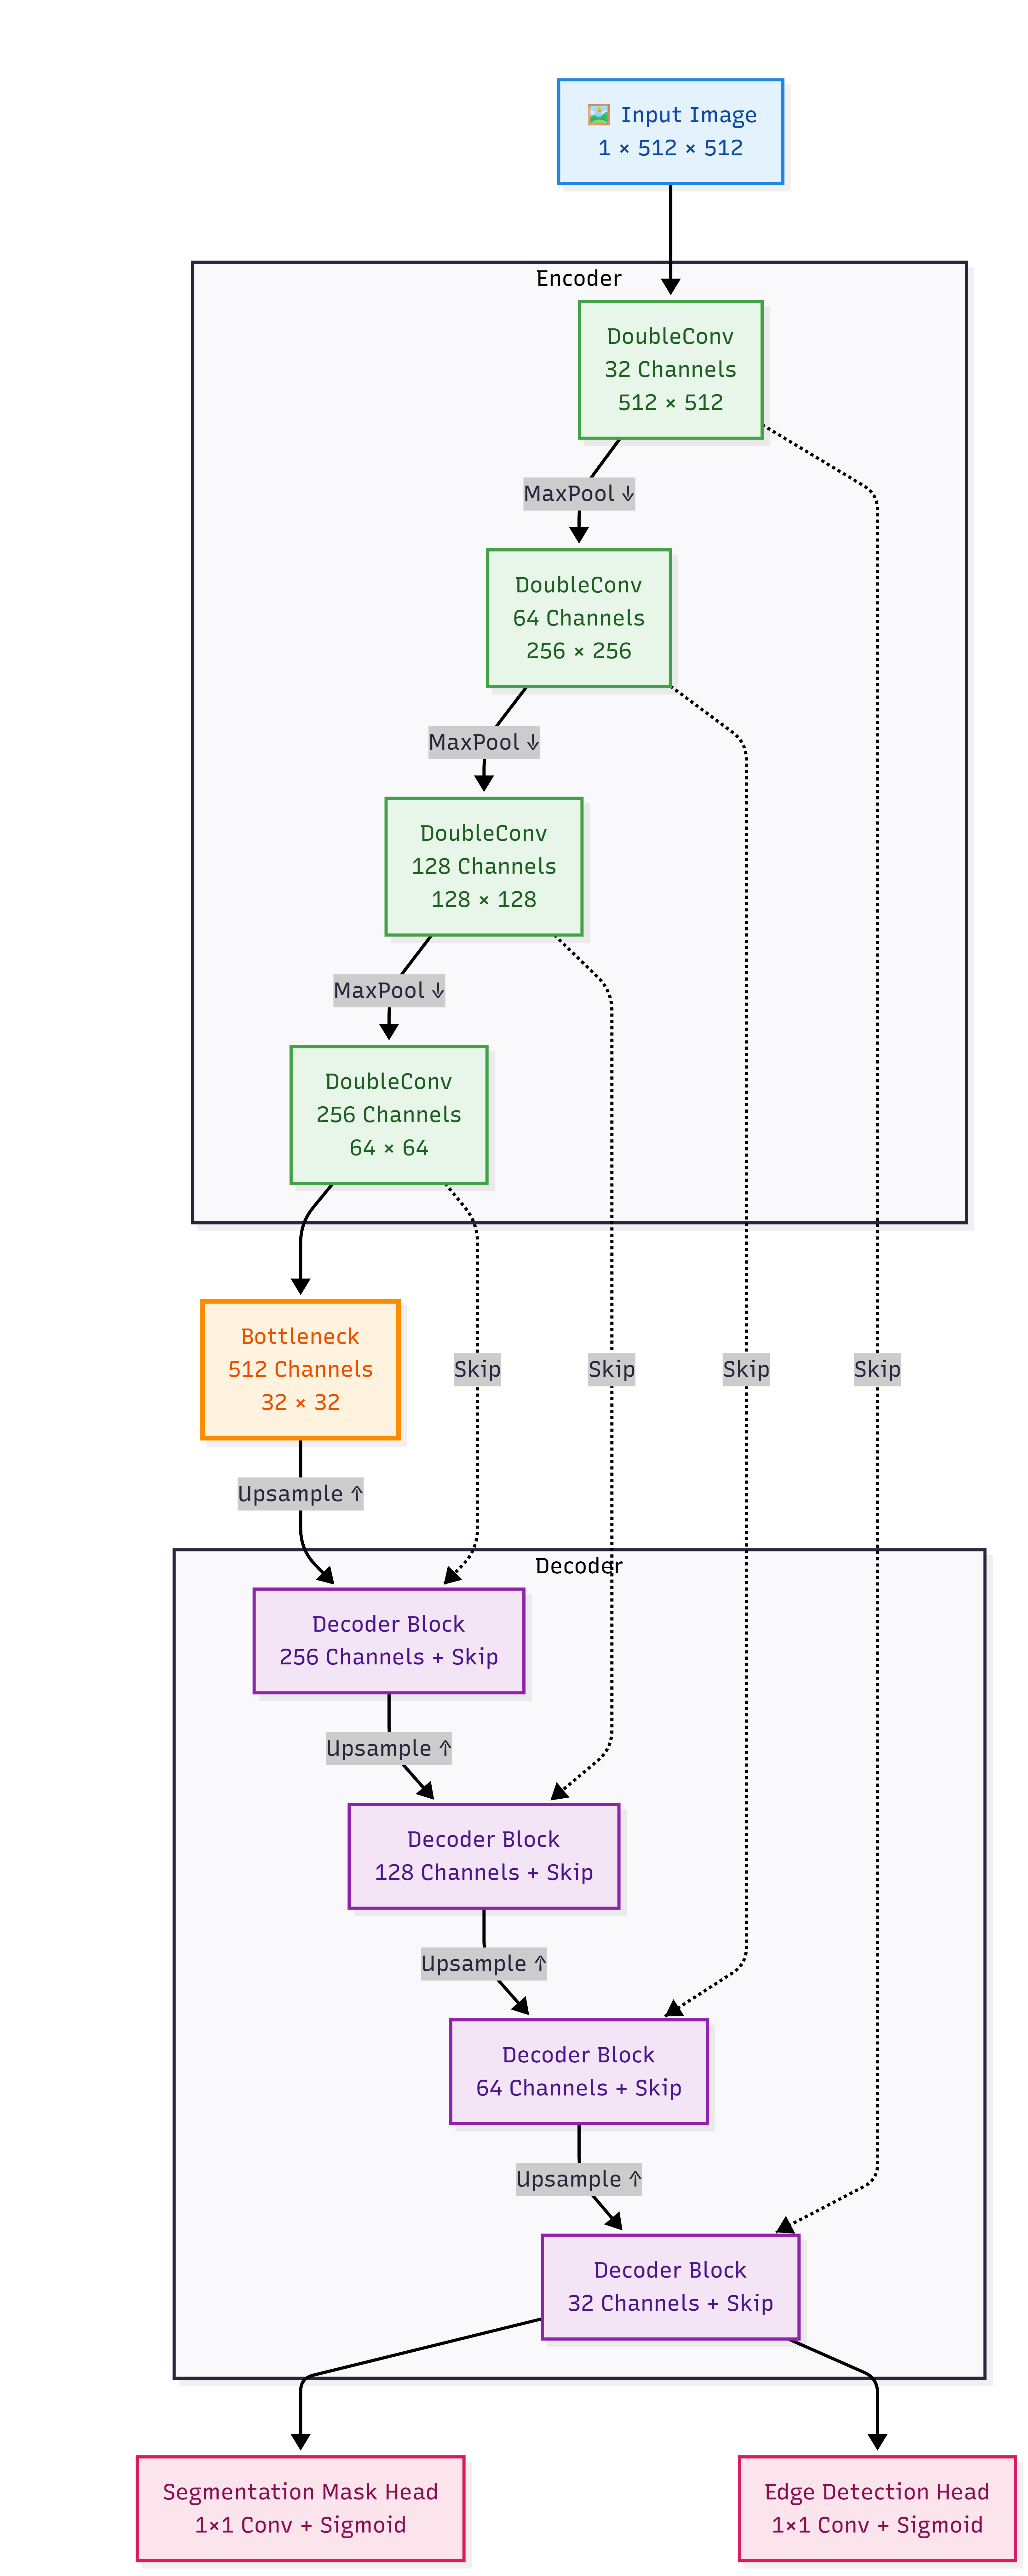
\includegraphics[
        width=\textwidth,
        height=0.92\textheight,
        keepaspectratio
    ]{Chapter3/unetarchitecture.png}
    \caption{Edge-Aware U-Net for lung segmentation with dual mask and edge output heads.}
    \label{fig:unet_arch}
\end{figure}
%------------------------------------------------------------------
\section{Normalization}
%------------------------------------------------------------------

All images are normalized using ImageNet statistics to align with the pretrained EfficientNet-B3 weights:

\[
\mu = [0.485,\ 0.456,\ 0.406], \quad \sigma = [0.229,\ 0.224,\ 0.225]
\]

The normalization is applied as the final step of every image transformation pipeline:

\begin{lstlisting}[style=pythonstyle, caption={Standard ImageNet normalization}]
transforms.Normalize([0.485, 0.456, 0.406],
                     [0.229, 0.224, 0.225])
\end{lstlisting}

Additionally, the patient age values have been clipped to the range $[0, 100]$ and divided by 100 to yield a normalized scalar in $[0,1]$, ensuring consistent numerical scale across metadata features.

For the segmentation model, images are normalized independently with mean $0.5$ and standard deviation $0.5$ since the U-Net is trained from scratch on grayscale inputs and does not use ImageNet pretrained weights.

%------------------------------------------------------------------
\section{Data Augmentation}
%------------------------------------------------------------------

Two distinct augmentation pipelines are used depending on the class frequency of each sample.

\subsection{Standard Augmentation (Common Classes)}

\begin{lstlisting}[style=pythonstyle, caption={Standard augmentation pipeline}]
common_transform = transforms.Compose([
    transforms.Resize((448, 448)),
    transforms.RandomHorizontalFlip(),
    transforms.ToTensor(),
    transforms.Normalize([0.485, 0.456, 0.406],
                         [0.229, 0.224, 0.225])
])
\end{lstlisting}

\subsection{Heavy Augmentation (Rare Classes)}

For rare pathologies such as Hernia, Fibrosis, and Emphysema, a heavier augmentation strategy is applied to synthetically increase sample diversity. This ensures that the model is able to generalize well even over diseases that aren't seen very often.

These are the Heavy transforms applied in order
\begin{enumerate}
    \item Resize
    \item Random Horizontal Flip
    \item Random Rotation (±20°)
    \item Random Resized Crop (Zoom 0.8–1.0)
    \item Random Affine Translation (10%)
    \item Color Jitter (Brightness, Contrast, Saturation)
    \item ToTensor 
    \item Normalize

\end{enumerate}

\subsection{SSL Augmentation (Two-View Contrastive)}

For OPTiML-inspired self-supervised pretraining, a two-view stochastic augmentation pipeline is applied to each image, generating a pair $(X_1, X_2)$. Gaussian noise is added as a final touch.

\subsection{Bounding Box Augmentation}

A critical design constraint for the localization pipeline is that all geometric augmentations (horizontal flip, random rotation, random crop, affine translation) must be \emph{removed} from the training transforms. These operations move pixels without updating the bounding box targets, corrupting the supervision signal. The localization training pipeline therefore uses only photometric transforms:

\begin{enumerate}
    \item Resize to $448 \times 448$
    \item ColorJitter (brightness $\pm 0.2$, contrast $\pm 0.2$, saturation $\pm 0.1$)
    \item ToTensor and ImageNet normalization
\end{enumerate}

\subsection{Segmentation Augmentation}

Joint augmentation is applied identically to the image and its corresponding mask to maintain spatial consistency. Only transforms that preserve the mask-pixel correspondence are used:

\begin{enumerate}
    \item Horizontal Flip (p=0.5)
    \item Rotation (±10°, constant border padding)
    \item Random Brightness/Contrast ($\pm 0.15$)
    \item Resize to $512 \times 512$
    \item Normalize (mean=0.5, std=0.5)
\end{enumerate}

A progressive unfreezing strategy is applied: the EfficientNet backbone is initially frozen so only the classification head is trained. At epoch 6, all backbone parameters are unfrozen and the learning rate is reduced to $10^{-5}$, this is in sync with the SSL+SL pretraining that was done which formed the backbone of bbox localization task.

For the SSL pretraining stage, \textbf{AdamW} is used with a lower weight decay to preserve spatial feature quality:

%------------------------------------------------------------------
\section{Loss Function}
%------------------------------------------------------------------

\subsection{Focal Loss for Supervised Classification}

Given the severe class imbalance in the NIH chest X-ray dataset, a \textbf{Multi-label Focal Loss} is used instead of usual Binary Cross-Entropy. The focal loss down-weights easy, well-classified examples and focuses learning on hard and misclassified samples:

\begin{equation}
\mathcal{L}_{\text{Focal}} = -\alpha \sum_{i} (1 - p_t)^{\gamma} \cdot \text{BCE}(\hat{y}_i, y_i)
\end{equation}

where $p_t = \sigma(\hat{y}_i)$ if $y_i = 1$, else $p_t = 1 - \sigma(\hat{y}_i)$, and $\alpha = 0.25$, $\gamma = 2.0$.

\subsection{OPTiML-Inspired SSL Loss}

The self-supervised pretraining stage uses a composite loss combining three components:

\subsubsection{Optimal Transport (OT) Structural Alignment~\cite{otcxr}}

Given two sets of dense patch embeddings $\mathbf{z}_1, \mathbf{z}_2 \in \mathbb{R}^{B \times HW \times D}$, a Sinkhorn-regularized optimal transport plan $\mathbf{T}$ is computed and the transport cost minimized.
\newline
Optimal Transport can be defined as the how can we align one geometry with the other with minimum cost possible so in our case we are using two augmented view so our problem is how can we align these two images probabilistically, now we can see it is somewhat similar to KL divergence but the key features that OT provides and is good for our use case is that it works at patch level and can align spatial structures whereas KL requires supports to overlap.
\begin{equation}
\mathcal{L}_{\text{OT}} = \sum_{i,j} T_{ij} \cdot C_{ij}, \quad C_{ij} = 1 - \cos\left(\mathbf{z}_{1,i},\ \mathbf{z}_{2,j}\right)
\end{equation}


\subsubsection{Variance Regularization~\cite{otcxr}}

Encourages representation diversity by penalizing collapsed feature dimensions:

\begin{equation}
\mathcal{L}_{\text{var}} = \mathbb{E}_d \left[\max\!\left(0,\ 1 - \sqrt{\mathrm{Var}_n(z_{n,d}) + \epsilon}\right)\right]
\end{equation}


\subsubsection{Covariance Regularization~\cite{otcxr}}

Decorrelates feature dimensions to reduce redundancy, following the Barlow Twins principle:

\begin{equation}
\mathcal{L}_{\text{cov}} = \frac{1}{D} \sum_{i \neq j} \left[\frac{(\mathbf{z}^\top \mathbf{z})_{ij}}{N-1}\right]^2
\end{equation}



\subsubsection{Total SSL Loss}

The complete SSL objective is:

\begin{equation}
\mathcal{L}_{\text{SSL}} = \mathcal{L}_{\text{OT}} + \lambda_{\text{var}} \cdot \mathcal{L}_{\text{var}} + \lambda_{\text{cov}} \cdot \mathcal{L}_{\text{cov}}
\end{equation}

with $\lambda_{\text{var}} = 0.1$ and $\lambda_{\text{cov}} = 0.01$.

\subsection{CIoU Loss for Bounding Box Regression}

Standard mean-squared error treats all coordinate errors equally regardless of box size. A \textbf{Combined Loss} of Complete IoU (CIoU) and Smooth-L1 is used instead:

\begin{equation}
\mathcal{L}_{\text{bbox}} = \mathcal{L}_{\text{CIoU}} + 0.5 \cdot \mathcal{L}_{\text{SmoothL1}}
\end{equation}

CIoU extends the standard IoU loss with a centre-distance penalty and an aspect-ratio consistency term:

\begin{equation}
\mathcal{L}_{\text{CIoU}} = 1 - \text{IoU} + \frac{d^2}{c^2} + \alpha v
\end{equation}

where $d^2$ is the squared Euclidean distance between predicted and target centres, $c^2$ is the squared diagonal of the smallest enclosing box, $v = \frac{4}{\pi^2}(\arctan\frac{w^{gt}}{h^{gt}} - \arctan\frac{\hat{w}}{\hat{h}})^2$ penalizes aspect-ratio mismatch, and $\alpha = v / (1 - \text{IoU} + v)$ is an adaptive weighting factor. The Smooth-L1 component provides stable gradient signal when predictions are far from targets.

\subsection{Segmentation Loss}

The total segmentation loss combines three terms:

\begin{equation}
\mathcal{L}_{\text{seg}} = \mathcal{L}_{\text{Dice}} + \mathcal{L}_{\text{BCE}}^{\text{boundary}} + \lambda_e \cdot \mathcal{L}_{\text{edge}}
\end{equation}

\paragraph{Dice Loss} addresses foreground-background imbalance by optimizing overlap directly:
\begin{equation}
\mathcal{L}_{\text{Dice}} = 1 - \frac{2\sum_i \hat{M}_i M_i + \epsilon}{\sum_i \hat{M}_i + \sum_i M_i + \epsilon}
\end{equation}

\paragraph{Boundary-Weighted BCE} amplifies the gradient signal at lung boundary pixels by upweighting them in the pixel-wise cross-entropy, encouraging sharper contours:
\begin{equation}
\mathcal{L}_{\text{BCE}}^{\text{boundary}} = \frac{1}{N}\sum_i (1 + \alpha \cdot E_i^{gt}) \cdot \text{BCE}(\hat{M}_i, M_i)
\end{equation}
where $E^{gt}$ is the ground-truth binary edge map and $\alpha = 5.0$ is the boundary amplification factor.

\paragraph{Edge Head Loss} directly supervises the auxiliary edge prediction branch:
\begin{equation}
\mathcal{L}_{\text{edge}} = \text{BCE}(\hat{E},\ E^{gt}), \quad \lambda_e = 0.3
\end{equation}

\subsection{Early Stopping}

To prevent overfitting, early stopping monitors validation AUC with a patience of 5 epochs and a minimum improvement delta of $10^{-4}$, this was removed to train SSL.

%------------------------------------------------------------------
\section{Post-Processing and Zone-Based Report Generation}
%------------------------------------------------------------------

\subsection{Segmentation Post-Processing}

Raw sigmoid probability maps from the U-Net are refined through a three-step pipeline before being used for zone extraction:

\begin{enumerate}
    \item \textbf{Threshold at 0.5} to produce a binary mask.
    \item \textbf{Morphological closing} (elliptical kernel, $k=7$, two iterations) to fill intra-lung holes introduced by vessels or airways and other silhouette overlap.
    \item \textbf{Connected-component filtering}: components smaller than 1,000 pixels are discarded; only the two largest remaining blobs (corresponding to the left and right lung) are retained.
\end{enumerate}

\subsection{Left/Right Lung Extraction and Zone Division}

The two boxes that surround the lungs are then assigned to left and right lungs by centroid $x$-coordinate following general convention: the patient's \emph{right} lung appears on the image \emph{left} (smaller centroid $x$), and the patient's \emph{left} lung appears on the image \emph{right} (larger centroid $x$).

Each lung bounding box is then divided into three equal horizontal thirds, yielding six zones that can be used for report generation:

\begin{table}[ht]
\centering
\caption{Anatomical zone nomenclature derived from segmented lung bounding boxes.}
\label{tab:zones}
\renewcommand{\arraystretch}{1.3}
\begin{tabular}{cll}
\toprule
\textbf{Zone Code} & \textbf{Full Name} & \textbf{Vertical Extent} \\
\midrule
RUZ & Right Upper Zone  & $y_1$ to $y_1 + \frac{H}{3}$ \\
RMZ & Right Middle Zone & $y_1 + \frac{H}{3}$ to $y_1 + \frac{2H}{3}$ \\
RLZ & Right Lower Zone  & $y_1 + \frac{2H}{3}$ to $y_2$ \\
LUZ & Left Upper Zone   & $y_1$ to $y_1 + \frac{H}{3}$ \\
LMZ & Left Middle Zone  & $y_1 + \frac{H}{3}$ to $y_1 + \frac{2H}{3}$ \\
LLZ & Left Lower Zone   & $y_1 + \frac{2H}{3}$ to $y_2$ \\
\bottomrule
\end{tabular}
\end{table}

Each detected disease is assigned to the zone with maximum bounding box intersection area, computed as the overlap between the disease bounding box (from the regressor) and each of the six zones, with the argmax zone selected.

\subsection{Structured Radiology Report Generation}

The final pipeline stage synthesizes outputs from all three models into a structured, template-driven report organized into five sections mirroring clinical reporting conventions:

\begin{enumerate}
    \item \textbf{Patient Information:} Study date, image filename, age, sex, and view position.
    \item \textbf{Findings Summary:} A concise list of all detected diseases with their classifier confidence scores.
    \item \textbf{Lung Field Assessment:} Reports whether each lung field was successfully segmented and provides bounding box coordinates for reference.
    \item \textbf{Zonal Analysis:} For each of the six zones (RUZ, RMZ, RLZ, LUZ, LMZ, LLZ), reports either the associated disease(s) with confidence or ``Appears normal.''
    \item \textbf{Impression:} A concise summary automatically detecting bilateral conditions (present in both left and right zones) and generating clinically phrased sentences.
\end{enumerate}

Rather than applying a global threshold to all disease probabilities, \textbf{per-class thresholds} are optimized on the validation set by maximizing macro-averaged F1 independently for each disease label. This is especially important for rare pathologies where the default 0.5 threshold produces trivially low recall.

\begin{lstlisting}[style=pythonstyle, caption={Sample generated radiology report (truncated)}]
======================================================================
                   CHEST X-RAY ANALYSIS REPORT
======================================================================
PATIENT INFORMATION
  Age: 69 years  |  Sex: Female  |  View: PA

FINDINGS SUMMARY
  Detected conditions (2):
    * Effusion      (confidence: 78.3%)
    * Atelectasis   (confidence: 65.1%)

ZONAL ANALYSIS
  Right Lower Zone  : Possible sign of Effusion (78.3%)
  Left Middle Zone  : Possible sign of Atelectasis (65.1%)
  [all other zones] : Appears normal

IMPRESSION
  * Effusion in the Right Lower Zone
  * Atelectasis in the Left Middle Zone
----------------------------------------------------------------------
  WARNING: AI-generated. Requires radiologist verification.
======================================================================
\end{lstlisting}

\begin{figure}[ht]
    \centering
    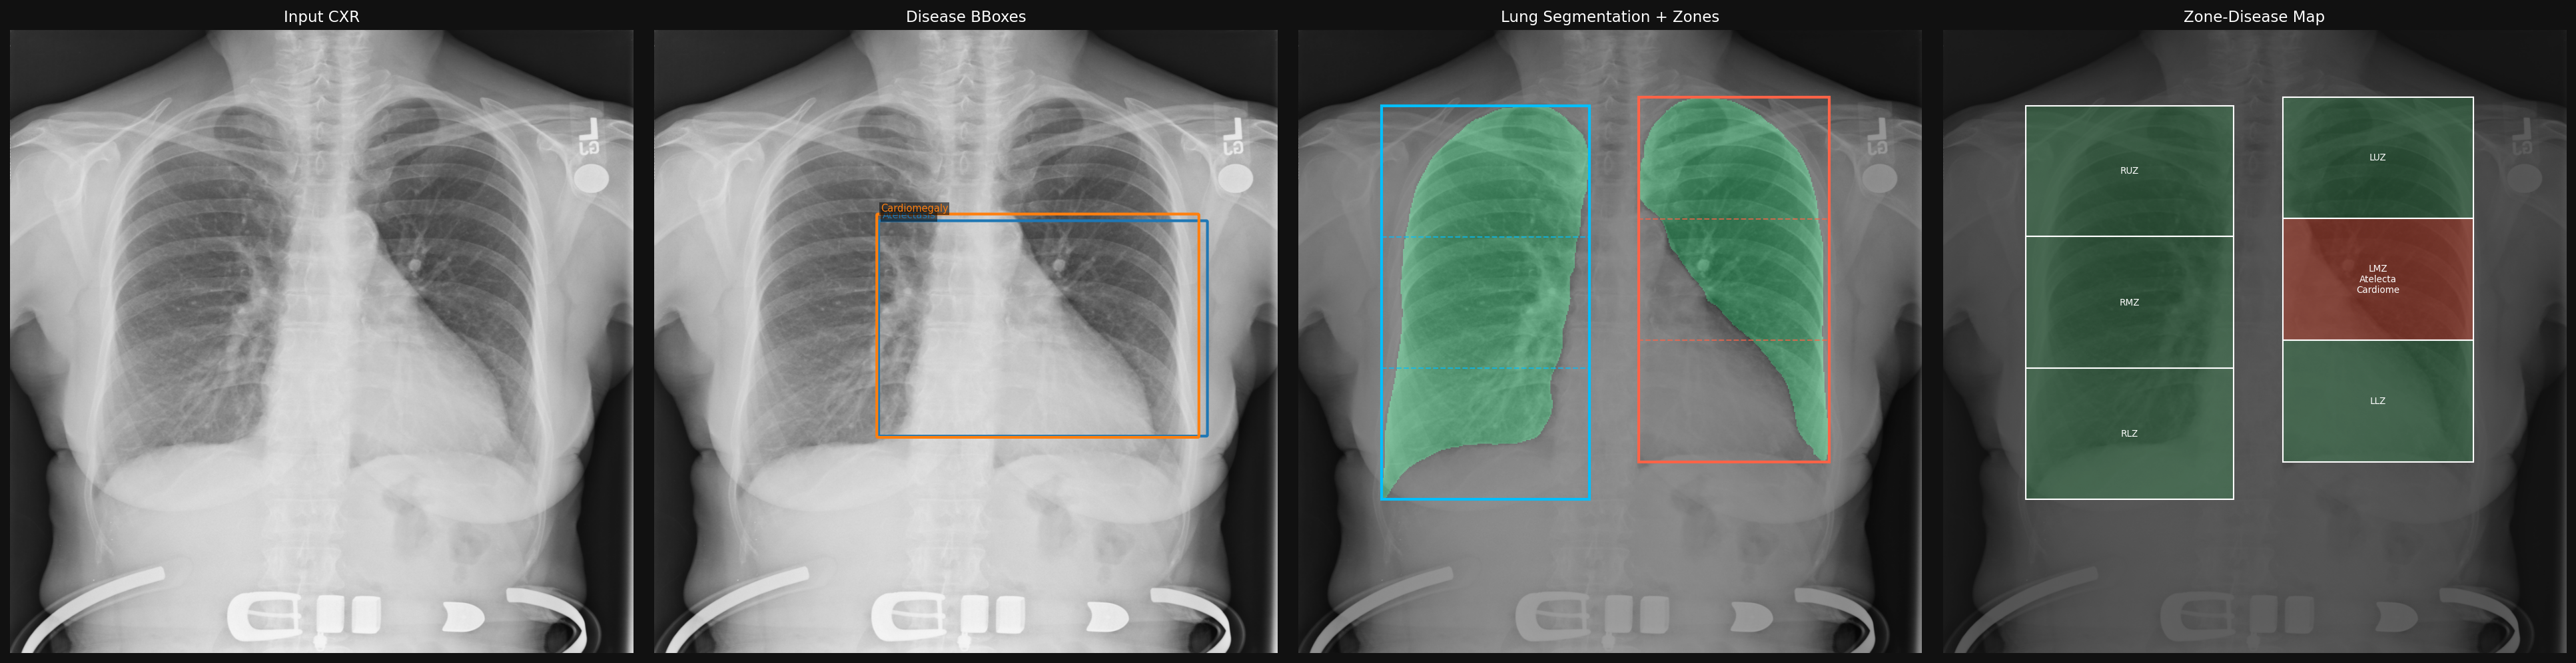
\includegraphics[
        width=\textwidth,
        height=0.99\textheight,
        keepaspectratio
    ]{Chapter3/pipeline_result.png}
    \caption{Four-panel visualisation of the complete inference pipeline on a sample NIH chest radiograph.}
    \label{fig:pipeline_viz}
\end{figure}

\begin{figure}[ht]
    \centering
    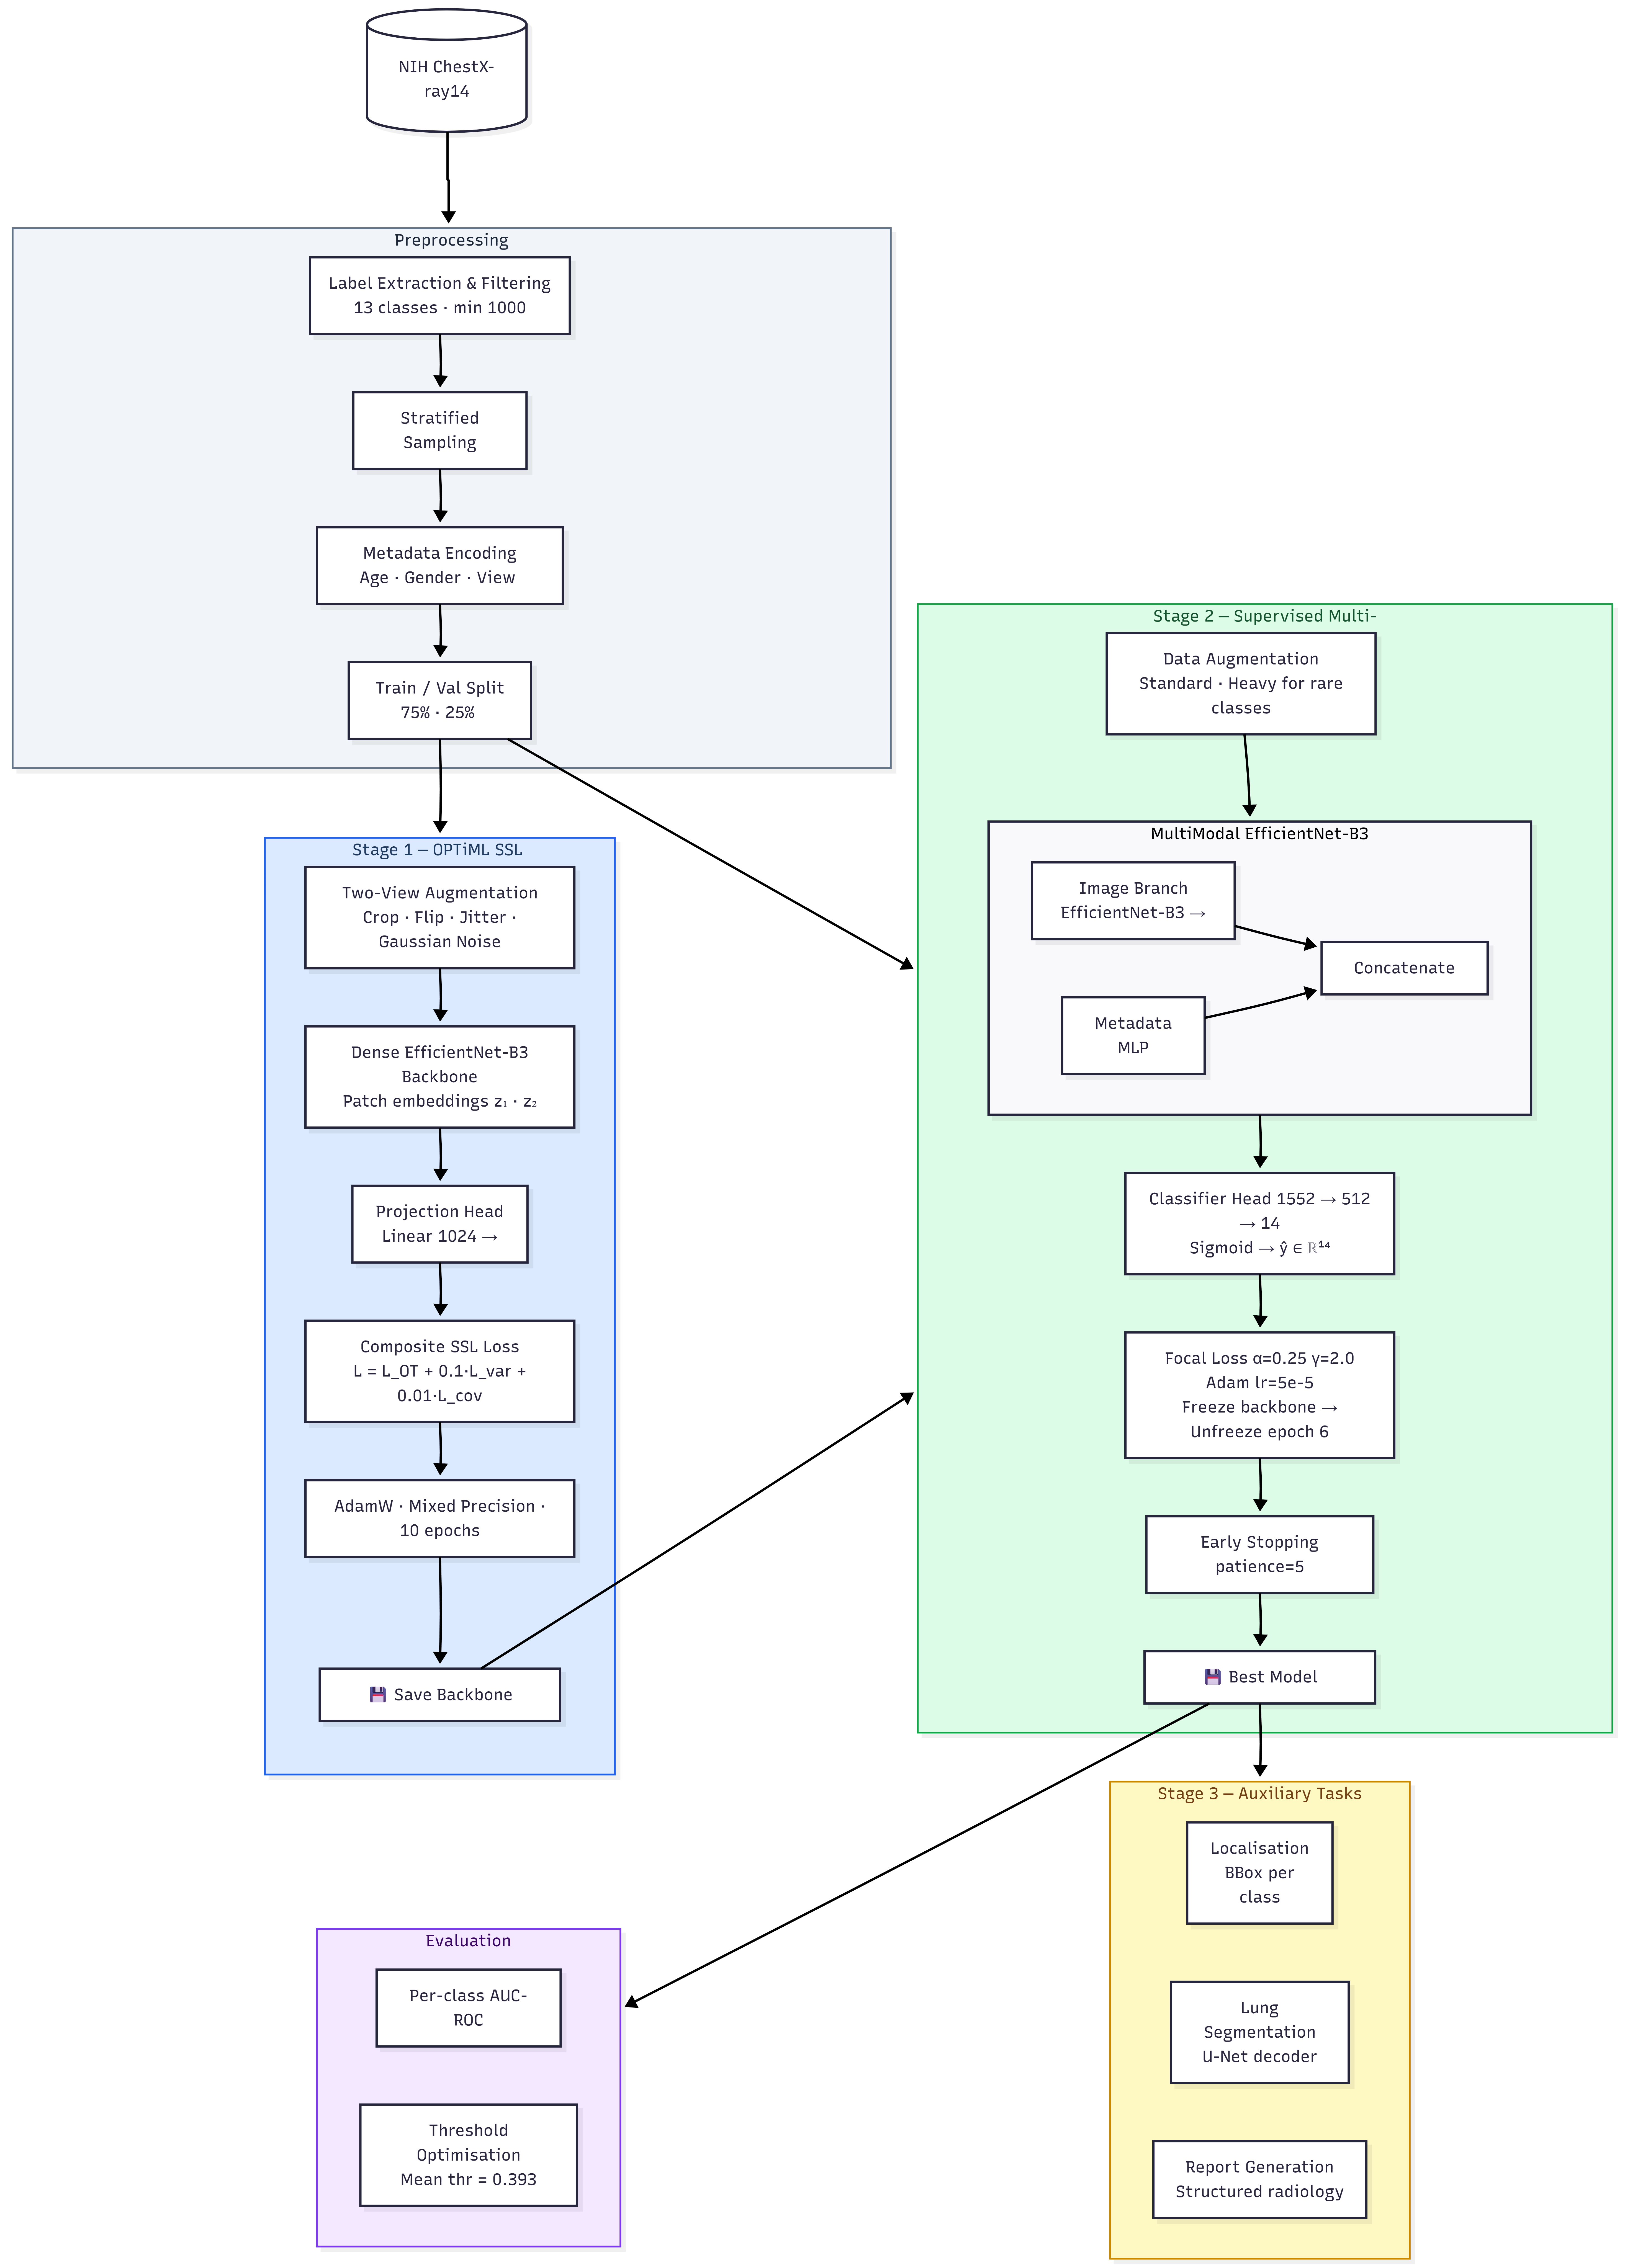
\includegraphics[width=\textwidth]{Chapter3/architecture_flow.png}
    \caption{Overall system architecture.}
    \label{fig:architecture}
\end{figure}
% ================================================================
% Chapter 4: Results and Analysis
% Included via \input{chapter4_results} in main.tex
% ================================================================
% Required packages (add to main.tex preamble if not present):
%   \usepackage{booktabs}
%   \usepackage{longtable}
%   \usepackage{array}
%   \usepackage{graphicx}
%   \usepackage{subcaption}
%   \usepackage{xcolor}
%   \usepackage{colortbl}
%   \usepackage{pgfplots}       % optional, for inline plots
%   \pgfplotsset{compat=1.18}
% ================================================================

\chapter{Results and Analysis}
\label{chap:results}

In this chapter we are focusing on the experimental results give by the SSL + SL model proposed and the impact of adding SSL as a pretraining step before. Results are reported for the SSL pretraining convergence, per-class AUC performance, threshold optimization, and auxiliary clinical tasks. A comparative analysis against baseline architectures is also provided.

% ------------------------------------------------------------------
\section{SSL Pretraining Convergence}
\label{sec:ssl_results}
% ------------------------------------------------------------------

The self-supervised pretraining was run for 3 epochs on the full training set without any disease labels. The composite loss $\mathcal{L}_{\text{SSL}} = \mathcal{L}_{\text{OT}} + 0.1\,\mathcal{L}_{\text{var}} + 0.01\,\mathcal{L}_{\text{cov}}$ was monitored across the epochs to assess representation learning convergence.

\begin{table}[ht]
\centering
\caption{OPTiML-inspired SSL pretraining loss per epoch.}
\label{tab:ssl_loss}
\renewcommand{\arraystretch}{1.3}
\begin{tabular}{cc}
\toprule
\textbf{Epoch} & \textbf{Average Loss} \\
\midrule
1  & 1.7447 \\
2  & 0.4308 \\
3  & 0.2672 \\
\bottomrule
\end{tabular}
\end{table}

The loss profile in Table~\ref{tab:ssl_loss} exhibits a sharp drop from 1.7447 at epoch 1 to 0.4308 at epoch 2, indicating rapid initial learning of coarse anatomical structure. The subsequent gradual decay from epoch 2 onward reflects the fine-grained alignment of spatial patch embeddings via the Sinkhorn optimal transport objective, combined with variance and covariance regularization. By epoch 3, the loss stabilises at 0.2672, suggesting the backbone has learned a compact, decorrelated representation of chest radiograph features before supervision learning.

% ------------------------------------------------------------------
\section{Supervised Multi-Label Classification}
\label{sec:supervised_results}
% ------------------------------------------------------------------

Following SSL pretraining, the EfficientNet-B3 backbone was fine-tuned under supervised multi-label classification using the Focal Loss objective. The model was trained for up to 50 epochs with early stopping (patience = 5). Training terminated at epoch 26 after the validation AUC failed to improve beyond the best recorded value of \textbf{0.8631}, the training AUC was reaching and crossing 0.91 but this overfitting was successfully contained by the early stopping mechanism, which halts training when validation performance degrades while training performance continues to improve.

\subsection{Training and Validation Curves}

\begin{figure}[ht]
    \centering
    \begin{subfigure}[b]{0.48\textwidth}
        \centering
        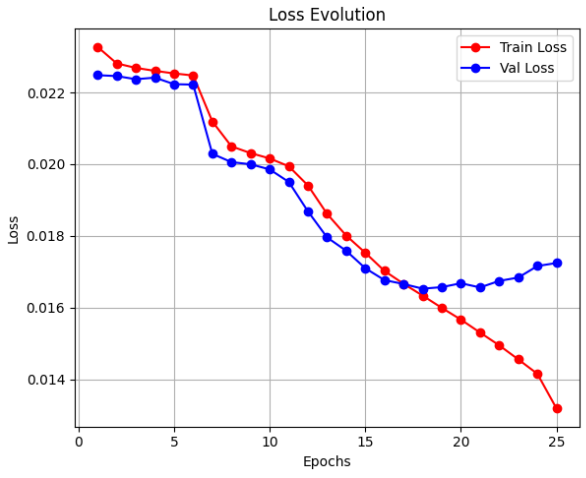
\includegraphics[width=\textwidth]{Chapter4/loss_auc_evolution.png}
        \caption{Training and validation loss over epochs.}
        \label{fig:loss_auc}
    \end{subfigure}
    \hfill
    \begin{subfigure}[b]{0.48\textwidth}
        \centering
        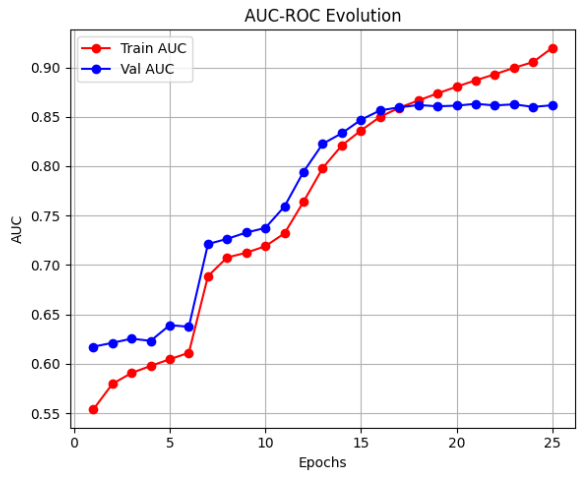
\includegraphics[width=\textwidth]{Chapter4/auc_with_control_line.png}
        \caption{AUC vs.\ epochs}
        \label{fig:auc_control}
    \end{subfigure}
    \caption{Learning curves for the supervised multi-label classification model.}
    \label{fig:learning_curves}
\end{figure}

The model achieved consistent improvement in both training and validation AUC across epochs, as shown in Figure~\ref{fig:learning_curves}. At epoch 25, the final recorded epoch before early stopping, the training metrics were:

\begin{itemize}
    \item \textbf{Train} Loss: 0.0132 $|$ AUC: 0.9198 $|$ F1: 0.4777
    \item \textbf{Val} Loss: 0.0172 $|$ AUC: 0.8617 $|$ F1: 0.3819
\end{itemize}

The train-validation AUC gap of approximately 0.058 indicates moderate overfitting in the later epochs, which the early stopping mechanism successfully contained. The validation loss increasing while training loss continued to decrease after epoch 20 triggered the early stopping counter, halting training at epoch 26.

\subsection{Per-Class AUC Performance}

Table~\ref{tab:per_class_auc} reports the AUC-ROC score for each of the 13 disease classes evaluated on the validation set, and Figure~\ref{fig:roc_curves} shows the corresponding ROC curves.

\begin{table}[ht]
\centering
\caption{Per-class AUC-ROC scores on the validation set (best model checkpoint).}
\label{tab:per_class_auc}
\renewcommand{\arraystretch}{1.3}
\begin{tabular}{lcc}
\toprule
\textbf{Pathology} & \textbf{AUC-ROC} & \textbf{Performance Band} \\
\midrule
Emphysema          & 0.9714 & \cellcolor{green!20}Excellent \\
Edema              & 0.9632 & \cellcolor{green!20}Excellent \\
Fibrosis           & 0.9403 & \cellcolor{green!20}Excellent \\
Pleural\_Thickening & 0.9350 & \cellcolor{green!20}Excellent \\
Consolidation      & 0.9301 & \cellcolor{green!20}Excellent \\
Pneumonia          & 0.8981 & \cellcolor{yellow!30}Good \\
Cardiomegaly       & 0.8824 & \cellcolor{yellow!30}Good \\
Pneumothorax       & 0.8729 & \cellcolor{yellow!30}Good \\
Effusion           & 0.8059 & \cellcolor{yellow!30}Good \\
Mass               & 0.7907 & \cellcolor{orange!20}Moderate \\
Atelectasis        & 0.7817 & \cellcolor{orange!20}Moderate \\
Nodule             & 0.7538 & \cellcolor{orange!20}Moderate \\
Infiltration       & 0.7011 & \cellcolor{orange!20}Moderate \\
\midrule
\textbf{Overall Average} & \textbf{0.8636} & \textbf{Good} \\
\bottomrule
\end{tabular}
\end{table}

The model achieves excellent discrimination (AUC $> 0.93$) for radiologically distinct pathologies with characteristic appearance: Emphysema (0.9714), Edema (0.9632), Fibrosis (0.9403), Pleural Thickening (0.9350), and Consolidation (0.9301). These diseases produce clearly separate regions on chest X-rays, making them easier to detect from image features alone.

Performance is moderate for diffuse or subtle findings like: Infiltration (0.7011), Nodule (0.7538), and Atelectasis (0.7817) which are similar visually with other pathologies and are subject to significant inter-observer variability in the source labels. This is consistent with observations across the literature on NIH ChestX-ray14.

\begin{figure}[ht]
    \centering
    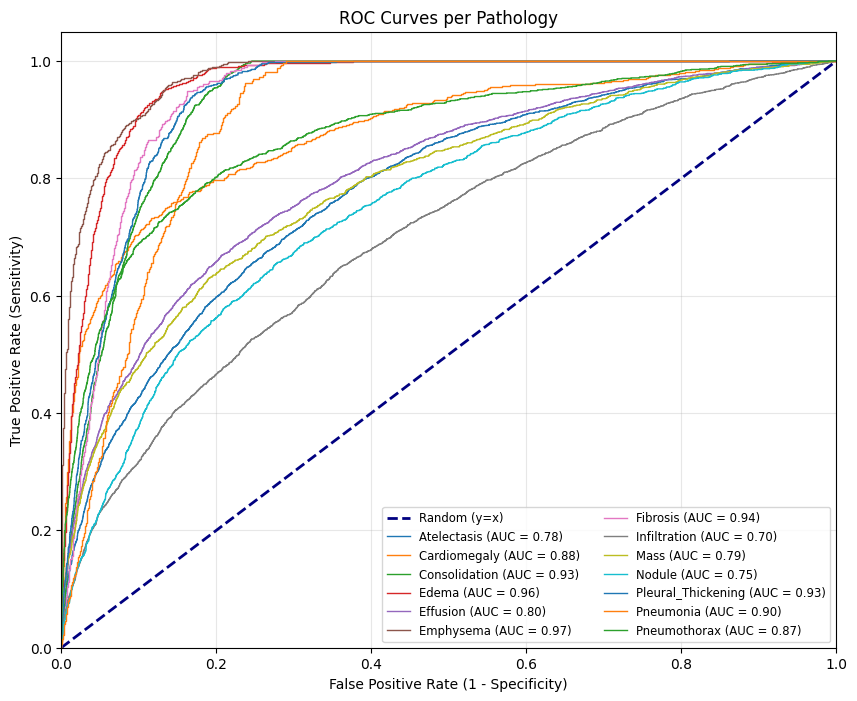
\includegraphics[width=0.85\textwidth]{Chapter4/roc_curves_per_pathology.png}
    \caption{ROC curves per pathology on the validation set. The dashed diagonal represents random classifier performance (AUC = 0.5).}
    \label{fig:roc_curves}
\end{figure}

% ------------------------------------------------------------------
\section{SSL Label Efficiency Analysis}
\label{sec:label_efficiency}
% ------------------------------------------------------------------

A key motivation for self-supervised pretraining is label efficiency which says that a model initialised from structure-aware representations requires fewer labelled examples to reach competitive performance. To test this, both the SSL-pretrained model (SL+SSL) and a supervised-only baseline (SL) were trained on progressively reduced fractions of the labelled training set: 100\%, 50\%, 25\%, and 10\%.

\begin{table}[ht]
\centering
\caption{Mean AUC-ROC at varying labelled data fractions for SL-only and SL+SSL models.}
\label{tab:label_efficiency}
\renewcommand{\arraystretch}{1.3}
\begin{tabular}{lcc}
\toprule
\textbf{Labelled Data Fraction} & \textbf{SL only} & \textbf{SL + SSL (proposed)} \\
\midrule
100\% & $\sim$0.860 & \textbf{0.8636} \\
50\%  & $\sim$0.860 & 0.8608          \\
25\%  & $\sim$0.850 & 0.8271          \\
10\%  & $\sim$0.830--0.840 & $>$0.80  \\
\bottomrule
\end{tabular}
\end{table}

\subsection{Key Observations}

\paragraph{At 100\% labels.} SL+SSL (0.8636) marginally outperforms the supervised-only baseline ($\sim$0.860), confirming that SSL pretraining provides a small but consistent benefit when all labelled data is available. The improvement is modest because the supervised model already has sufficient signal to learn discriminative features from the full dataset.

\paragraph{At 50\% labels.} SL+SSL (0.8608) achieves performance essentially equivalent to SL trained on the full 100\% dataset ($\sim$0.860). This is the most practically significant result: \textbf{SSL pretraining effectively halves the labelled data requirement} with no meaningful loss in AUC. For a medical imaging context where expert annotation is expensive and scarce, this represents a substantial reduction in labelling cost.

\paragraph{At 25\% labels.} Both models degrade, but SL+SSL (0.8271) falls further than SL ($\sim$0.850). This counter-intuitive result suggests that at very low label counts, the SSL-pretrained backbone's inductive biases may not align well with the fine-grained discriminative signal available from only 25\% of labels, while the supervised model's simpler initialisation adapts more directly.

\paragraph{At 10\% labels.} Both models maintain AUC above 0.80, which is notable given the extreme label reduction. SL+SSL does not demonstrate a clear advantage here; the two models converge to similar performance. At this scale, the bottleneck is likely the label set itself rather than the initialisation quality: with so few positive examples per class, neither model has sufficient signal to reliably separate the disease-specific features learned during pretraining.

\subsection{Interpretation}

The label efficiency results are consistent with the broader SSL literature: pretraining benefits are largest in the moderate data regime (around 50\% of full labels) and diminish at both extremes. At full data, supervised training alone approaches the SSL ceiling. At very low data, the SSL representations may be over-specified for the pretraining task (patch-level structural alignment) and under-specified for the fine-grained class boundaries needed for rare-class discrimination.

The practical takeaway is that \textbf{SL+SSL trained on 50\% of labels matches SL trained on 100\%}, making the proposed pipeline particularly attractive for settings where annotation budgets are constrained. The 25\% and 10\% regimes would benefit from a larger SSL pretraining corpus or a longer pretraining schedule to push the representations closer to the downstream task distribution.

% ------------------------------------------------------------------
\section{Threshold Optimisation}
\label{sec:threshold}
% ------------------------------------------------------------------

The default classification threshold of 0.5 is suboptimal for imbalanced multi-label problems. A per-class threshold search over the range $[0.0, 1.0]$ with step 0.01 was performed on the validation set to maximise the per-class F1 score.

\subsection{Overall Impact}

\begin{table}[ht]
\centering
\caption{Overall F1 improvement from per-class threshold optimisation.}
\label{tab:threshold_overall}
\renewcommand{\arraystretch}{1.3}
\begin{tabular}{lccc}
\toprule
\textbf{Metric} & \textbf{Default (0.5)} & \textbf{Optimised} & \textbf{Improvement} \\
\midrule
Macro F1 & 0.3444 & 0.5103 & \textbf{+0.1660} \\
Micro F1 & 0.4232 & 0.5258 & \textbf{+0.1026} \\
\bottomrule
\end{tabular}
\end{table}

As shown in Table~\ref{tab:threshold_overall}, threshold optimisation yields a substantial improvement of \textbf{+0.166} in Macro F1 and \textbf{+0.103} in Micro F1. The consistent downward shift of optimal thresholds below 0.5 (mean optimal threshold = 0.393) suggests the model is systematically under-confident in its positive predictions a common consequence of class imbalance and Focal Loss down-weighting.

\subsection{Per-Class Threshold Analysis}

\begin{table}[ht]
\centering
\caption{Per-class threshold optimisation results.}
\label{tab:threshold_perclass}
\renewcommand{\arraystretch}{1.3}
\begin{tabular}{lccccr}
\toprule
\textbf{Pathology} & \textbf{Def.\ Thr.} & \textbf{Opt.\ Thr.} & \textbf{Def.\ F1} & \textbf{Opt.\ F1} & \textbf{$\Delta$F1} \\
\midrule
Atelectasis        & 0.500 & 0.390 & 0.4377 & 0.5384 & +0.1007 \\
Cardiomegaly       & 0.500 & 0.370 & 0.4532 & 0.5373 & +0.0840 \\
Consolidation      & 0.500 & 0.400 & 0.3935 & 0.5715 & +0.1780 \\
Edema              & 0.500 & 0.400 & 0.3531 & 0.5806 & +0.2275 \\
Effusion           & 0.500 & 0.420 & 0.5573 & 0.5921 & +0.0348 \\
Emphysema          & 0.500 & 0.440 & 0.6441 & 0.6807 & +0.0366 \\
Fibrosis           & 0.500 & 0.350 & 0.0000 & 0.3973 & +0.3973 \\
Infiltration       & 0.500 & 0.410 & 0.4380 & 0.5327 & +0.0947 \\
Mass               & 0.500 & 0.400 & 0.2812 & 0.4531 & +0.1719 \\
Nodule             & 0.500 & 0.400 & 0.1872 & 0.4241 & +0.2369 \\
Pleural\_Thickening & 0.500 & 0.390 & 0.1919 & 0.5085 & +0.3166 \\
Pneumonia          & 0.500 & 0.320 & 0.0000 & 0.2395 & +0.2395 \\
Pneumothorax       & 0.500 & 0.420 & 0.5393 & 0.5784 & +0.0391 \\
\midrule
\textbf{Average}   & 0.500 & \textbf{0.393} & 0.3444 & \textbf{0.5103} & \textbf{+0.1660} \\
\bottomrule
\end{tabular}
\end{table}

Table~\ref{tab:threshold_perclass} reveals particularly large gains for classes that scored zero F1 at the default threshold: \textbf{Fibrosis} (+0.397) and \textbf{Pneumonia} (+0.240) were entirely suppressed at threshold 0.5 due to their low positive sample counts (408 and 328 respectively), and only become detectable after the threshold is lowered. Similarly, \textbf{Pleural Thickening} (+0.317) and \textbf{Nodule} (+0.237) see dramatic improvements, confirming that rare-class predictions are systematically under-confident.

The smallest gains are observed for already high performing classes: \textbf{Effusion} (+0.035) and \textbf{Emphysema} (+0.037), which already achieve high F1 at the default threshold.

\begin{figure}[ht]
    \centering
    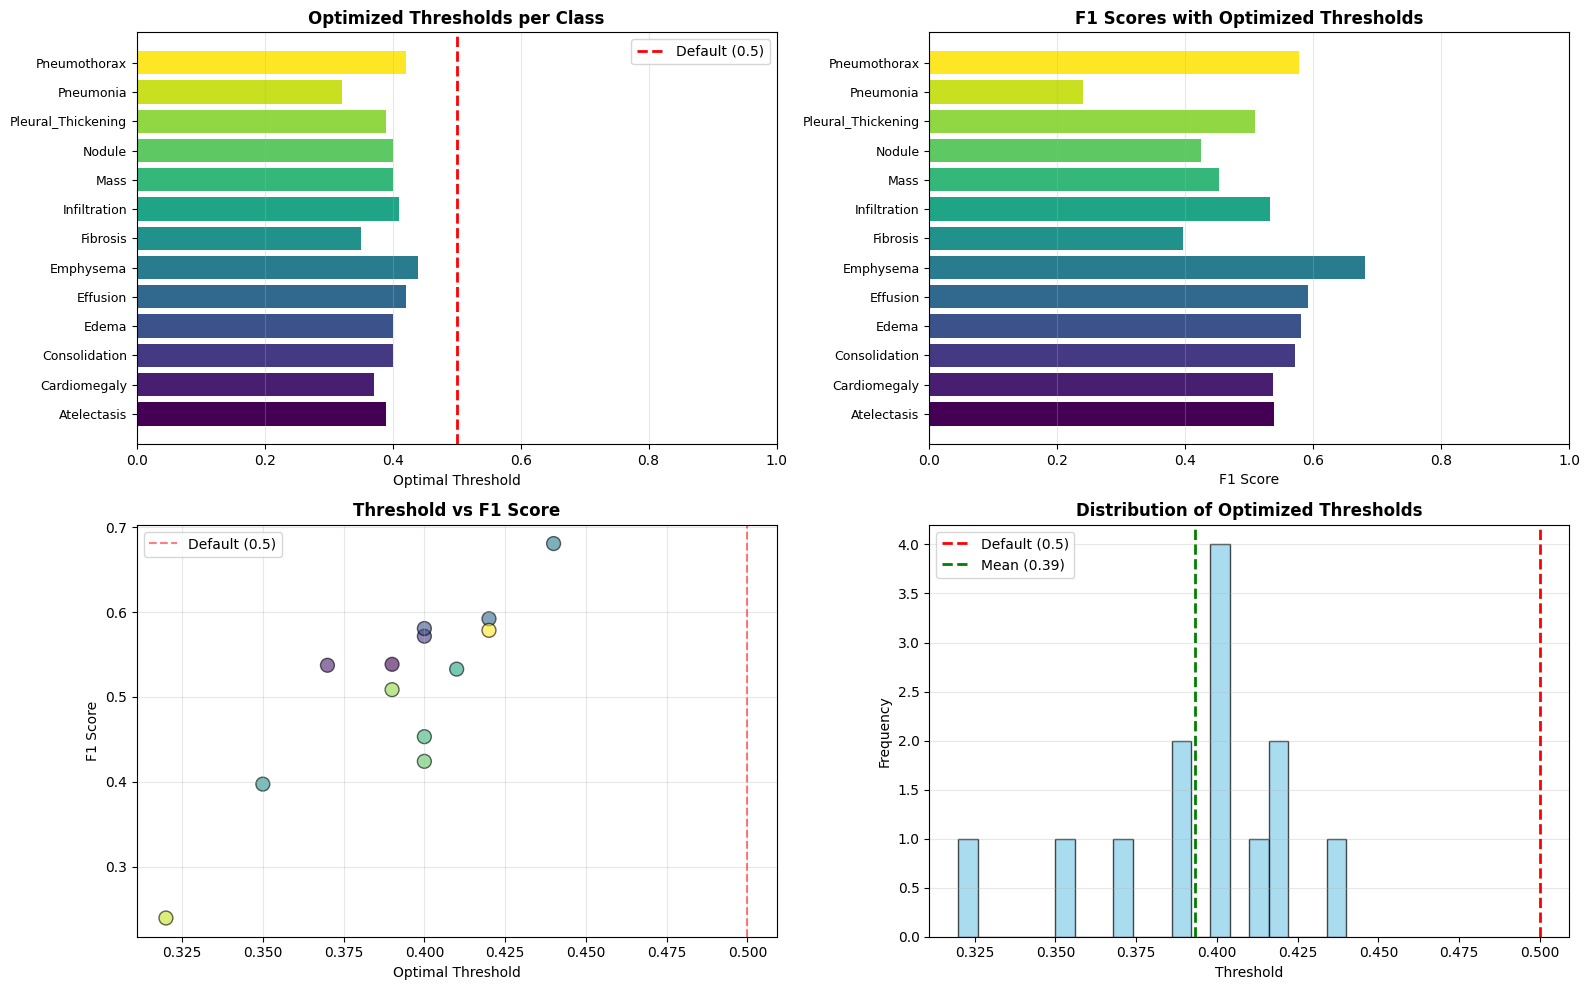
\includegraphics[width=0.95\textwidth]{Chapter4/threshold_optimization_results.png}
    \caption{Threshold optimisation results: (top-left) optimal thresholds per class, (top-right) F1 scores with optimised thresholds, (bottom-left) threshold vs.\ F1 scatter, (bottom-right) distribution of optimal thresholds.}
    \label{fig:threshold_opt}
\end{figure}

The distribution of optimised thresholds (Figure~\ref{fig:threshold_opt}, bottom-right) is concentrated in the range $[0.32, 0.44]$, well below the default 0.5. This is a direct artefact of the Focal Loss training objective, which suppresses easy negative loss contributions, causing the model to output lower raw probabilities for positive cases. Threshold calibration is therefore a necessary post-processing step for any deployment of this model. Moreover we are looking for peaks in probabilities as they tend to show anomalies so threshold optimisation tells us local maximas necessary for successful detection.

% ------------------------------------------------------------------
\section{Representation Quality: t-SNE Visualisation}
\label{sec:tsne}
% ------------------------------------------------------------------

To qualitatively assess the structure of the learned representations, t-SNE projections of the EfficientNet-B3 feature embeddings are visualised on the validation set under two grouping schemes.

\begin{figure}[ht]
    \centering
    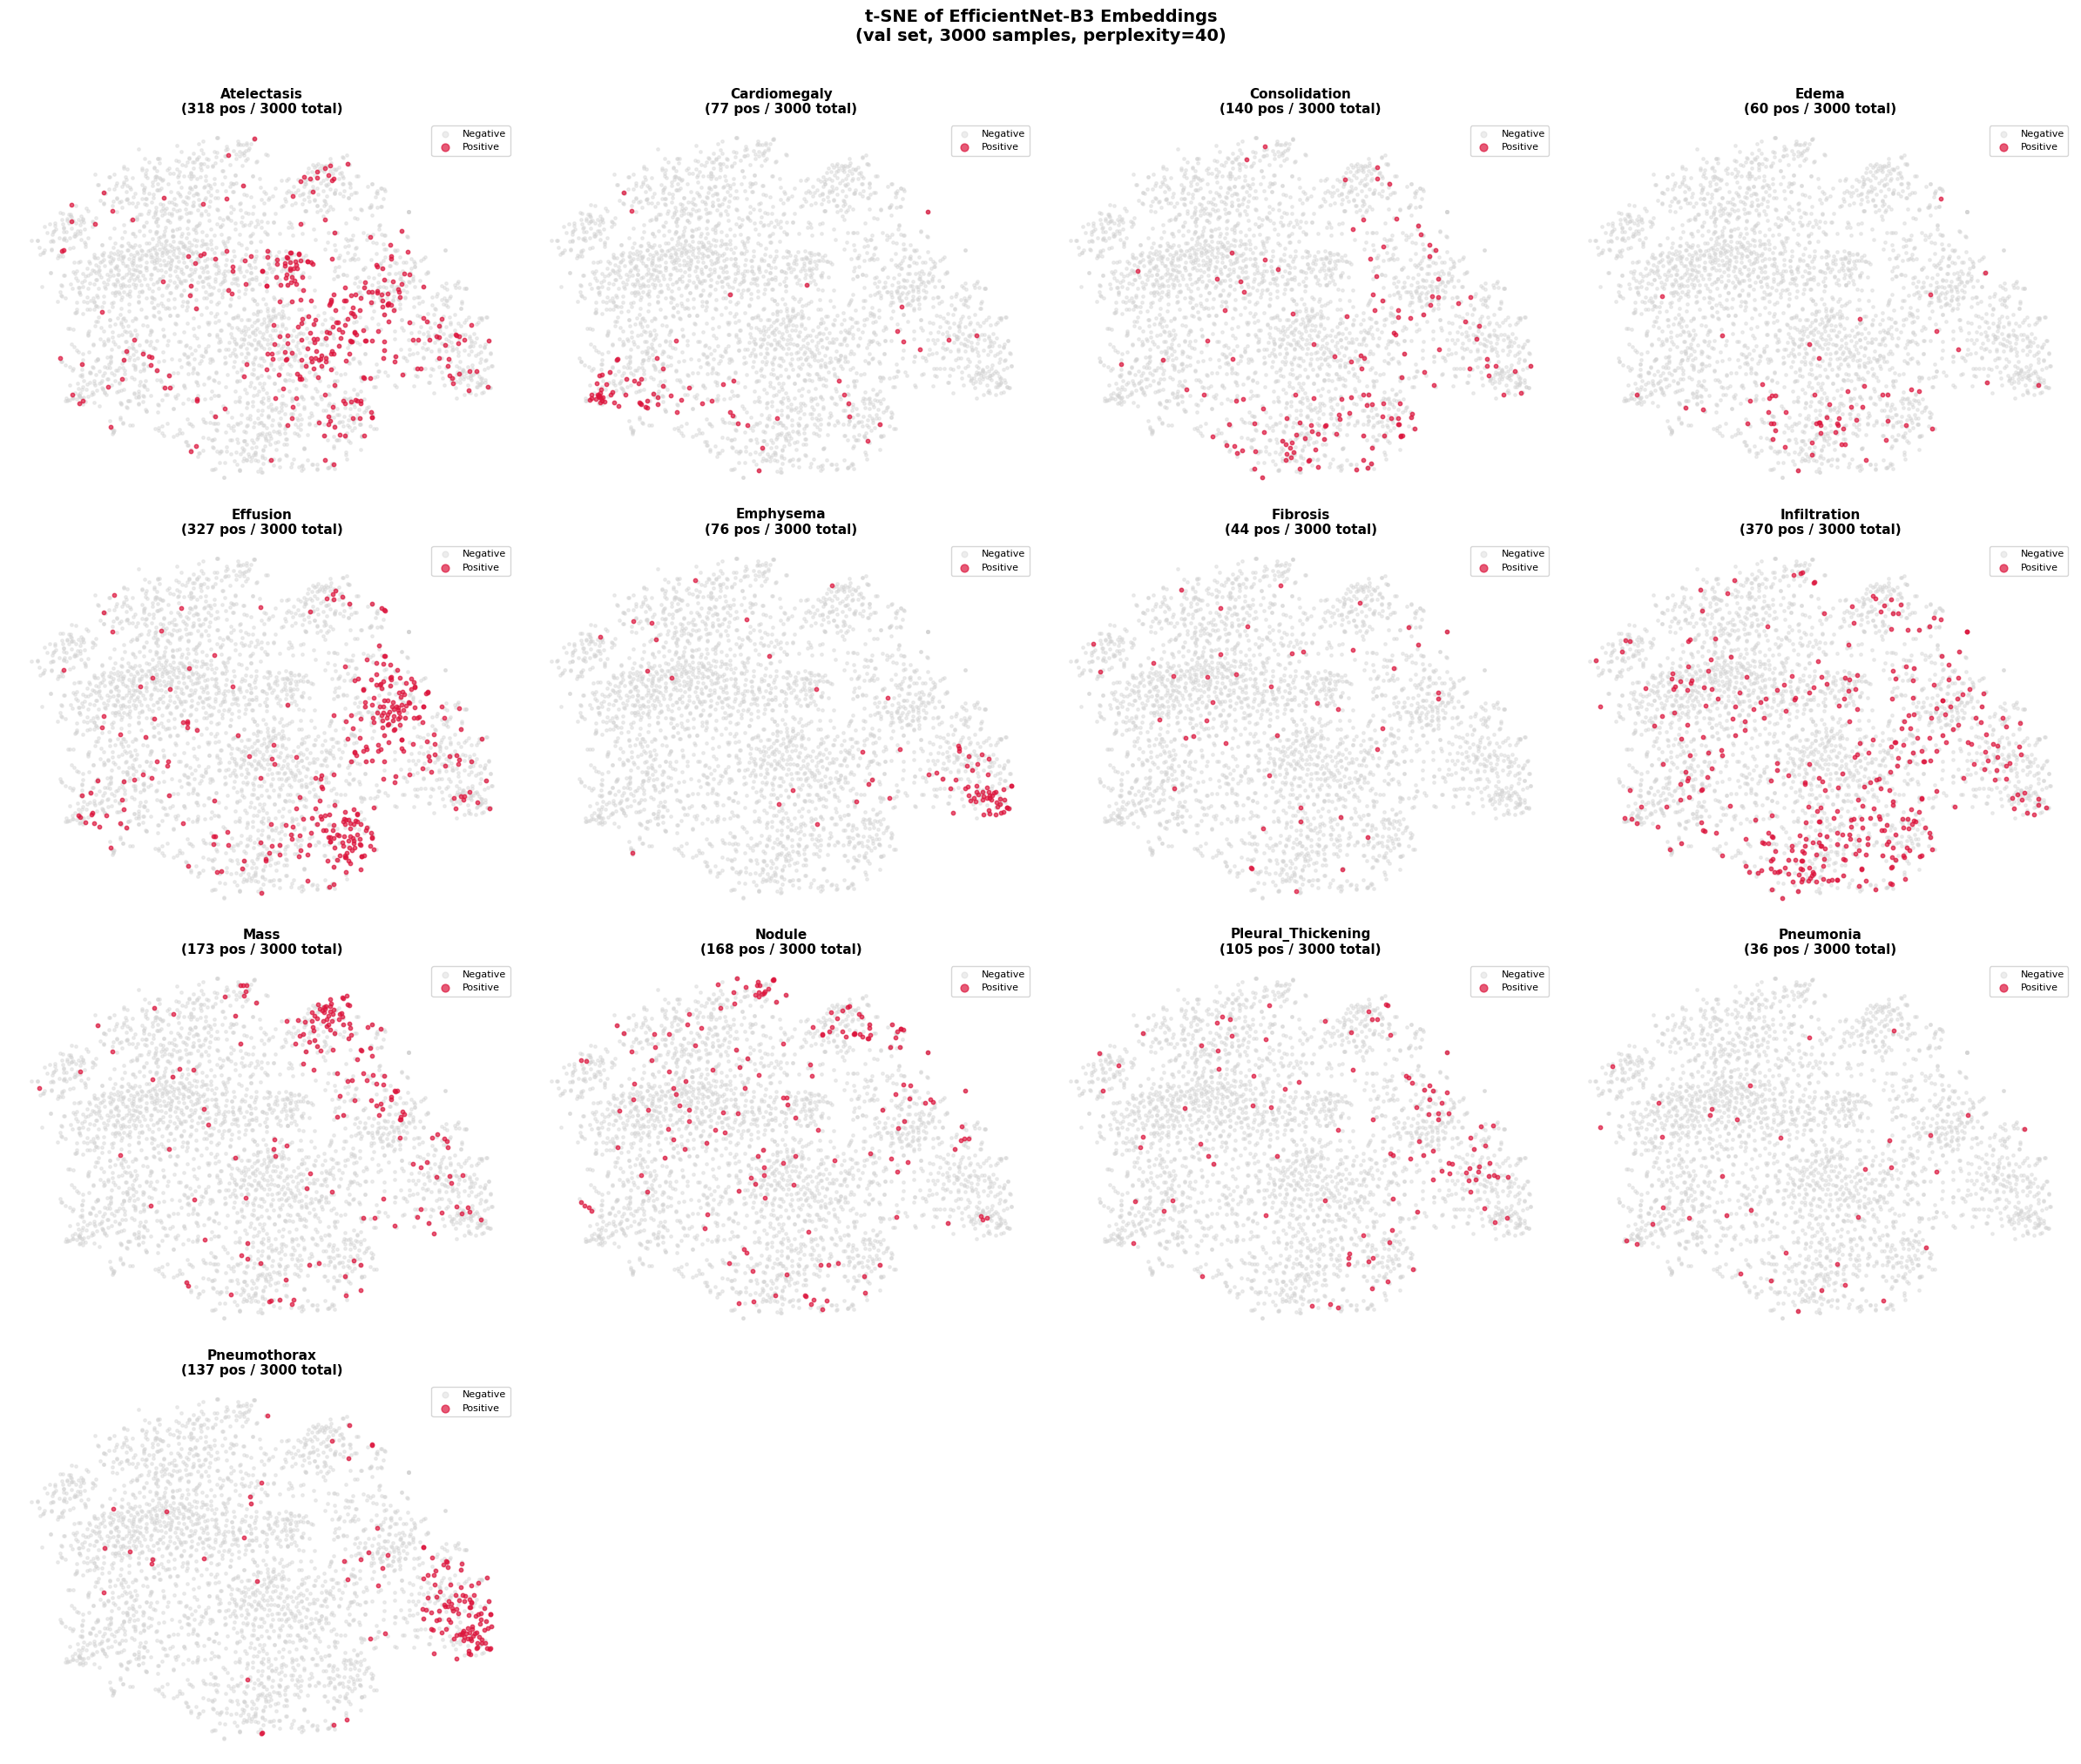
\includegraphics[width=\textwidth]{Chapter4/attachments/tsne_disease_vs_normal.png}
    \caption{t-SNE projection of validation embeddings coloured by individual disease label versus Normal. Each subplot corresponds to one disease class, showing the degree of separation between positive cases (coloured) and Normal cases (gray).}
    \label{fig:tsne_per_disease}
\end{figure}
\FloatBarrier

\begin{figure}[ht]
    \centering
    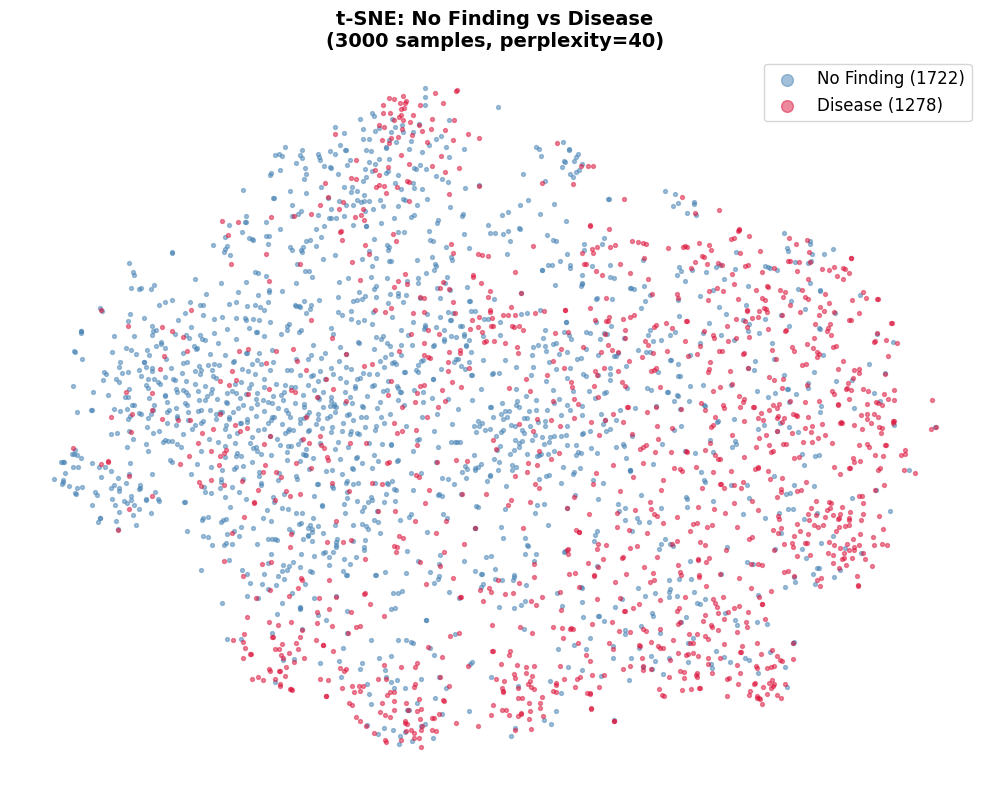
\includegraphics[width=0.65\textwidth]{Chapter4/attachments/tsne_anydisease_vs_normal.png}
    \caption{t-SNE projection coloured by any disease present versus Normal. Positive cases (any pathology) are shown in one colour; Normal cases in another.}
    \label{fig:tsne_any_vs_normal}
\end{figure}

Figure~\ref{fig:tsne_per_disease} shows per-disease subplots: radiologically distinct pathologies such as Emphysema, Cardiomegaly, and Edema form tight, well-separated clusters relative to Normal, consistent with their high per-class AUC scores. Diffuse pathologies such as Infiltration and Atelectasis show greater overlap with the Normal distribution, reflecting the inherent ambiguity in their visual presentation. Figure~\ref{fig:tsne_any_vs_normal} shows that at a coarse level the model broadly separates diseased from normal radiographs, confirming that the SSL pretraining has instilled a global sense of anatomical normality into the feature space before supervised fine-tuning.

% ------------------------------------------------------------------
\section{Comparative Baseline Analysis}
\label{sec:baselines}
% ------------------------------------------------------------------

To contextualise the contribution of the SSL pretraining, the final model is compared against several baseline architectures trained under fully supervised conditions on the same dataset and split.

\begin{table}[ht]
\centering
\caption{Comparison of mean AUC-ROC across baseline architectures and the proposed model.}
\label{tab:baselines}
\renewcommand{\arraystretch}{1.4}
\begin{tabular}{lcc}
\toprule
\textbf{Model} & \textbf{Mean AUC-ROC} & \textbf{Notes} \\
\midrule
ResNet-50 (supervised)          & 0.60  & Fully supervised, no SSL \\
DenseNet-121 (supervised)       & 0.77  & Fully supervised, no SSL \\
ViT / Swin Transformer          & 0.80             & After 7 epochs\\
EfficientNet-B3 (supervised)    & 0.85  & Multimodal, no SSL pretraining \\
\midrule
\rowcolor{green!15}
\textbf{EfficientNet-B3 + OPTiML SSL (proposed)} & \textbf{0.8636} & \textbf{SSL + multimodal fusion} \\
\bottomrule
\end{tabular}
\end{table}

As shown in Table~\ref{tab:baselines}, the proposed SSL pretraining provides a consistent improvement over the equivalent supervised-only EfficientNet-B3 baseline. ResNet-50 and DenseNet-121 serve as lightweight reference points, confirming that architectural capacity and pretraining strategy both contribute meaningfully to classification performance. The ViT/Swin result (0.80 after 7 epochs with partially frozen layers) suggests that transformer-based models require longer fine-tuning schedules to reach competitive performance on this dataset but from the trend in AUC across epochs the model has high chance of exceeding the CNN performance as expected.

The improvement from supervised EfficientNet-B3 to the SSL-augmented variant, while miniscule, is consistent with the hypothesis that structure-aware, decorrelated representations learned without label noise provide a better initialisation point for fine-tuning. The SSL pretraining enforces anatomical consistency across augmented views through the Sinkhorn optimal transport objective, which appears to improve generalisation on moderate and rare classes in particular.

% ------------------------------------------------------------------
\section{Auxiliary Task Results}
\label{sec:auxiliary}
% ------------------------------------------------------------------

In addition to the primary classification objective, two additional clinical tasks were evaluated to demonstrate the extensibility and spatial quality of the learned representations: disease localisation via bounding box regression and lung region segmentation.

\subsection{Disease Localisation}

Bounding box regression was trained for 60 epochs with early stopping (patience = 8). Training halted at epoch 34 with the best validation mean IoU of \textbf{0.2110} restored from the best checkpoint.

\begin{table}[ht]
\centering
\caption{Bounding box regression training summary at early stopping (epoch 34).}
\label{tab:bbox_training}
\renewcommand{\arraystretch}{1.3}

\begin{tabular}{lcccc}
\toprule
\textbf{Split} & \textbf{Loss} & \textbf{mIoU} & \textbf{IoU@0.25} & \textbf{IoU@0.50} \\
\midrule
Train & 0.7518 & 0.3056 & 0.466 & 0.270 \\
Val   & 0.9392 & 0.2063 & 0.336 & 0.161 \\
\bottomrule
\end{tabular}
\end{table}

\FloatBarrier
\begin{figure}[ht]
    \centering
    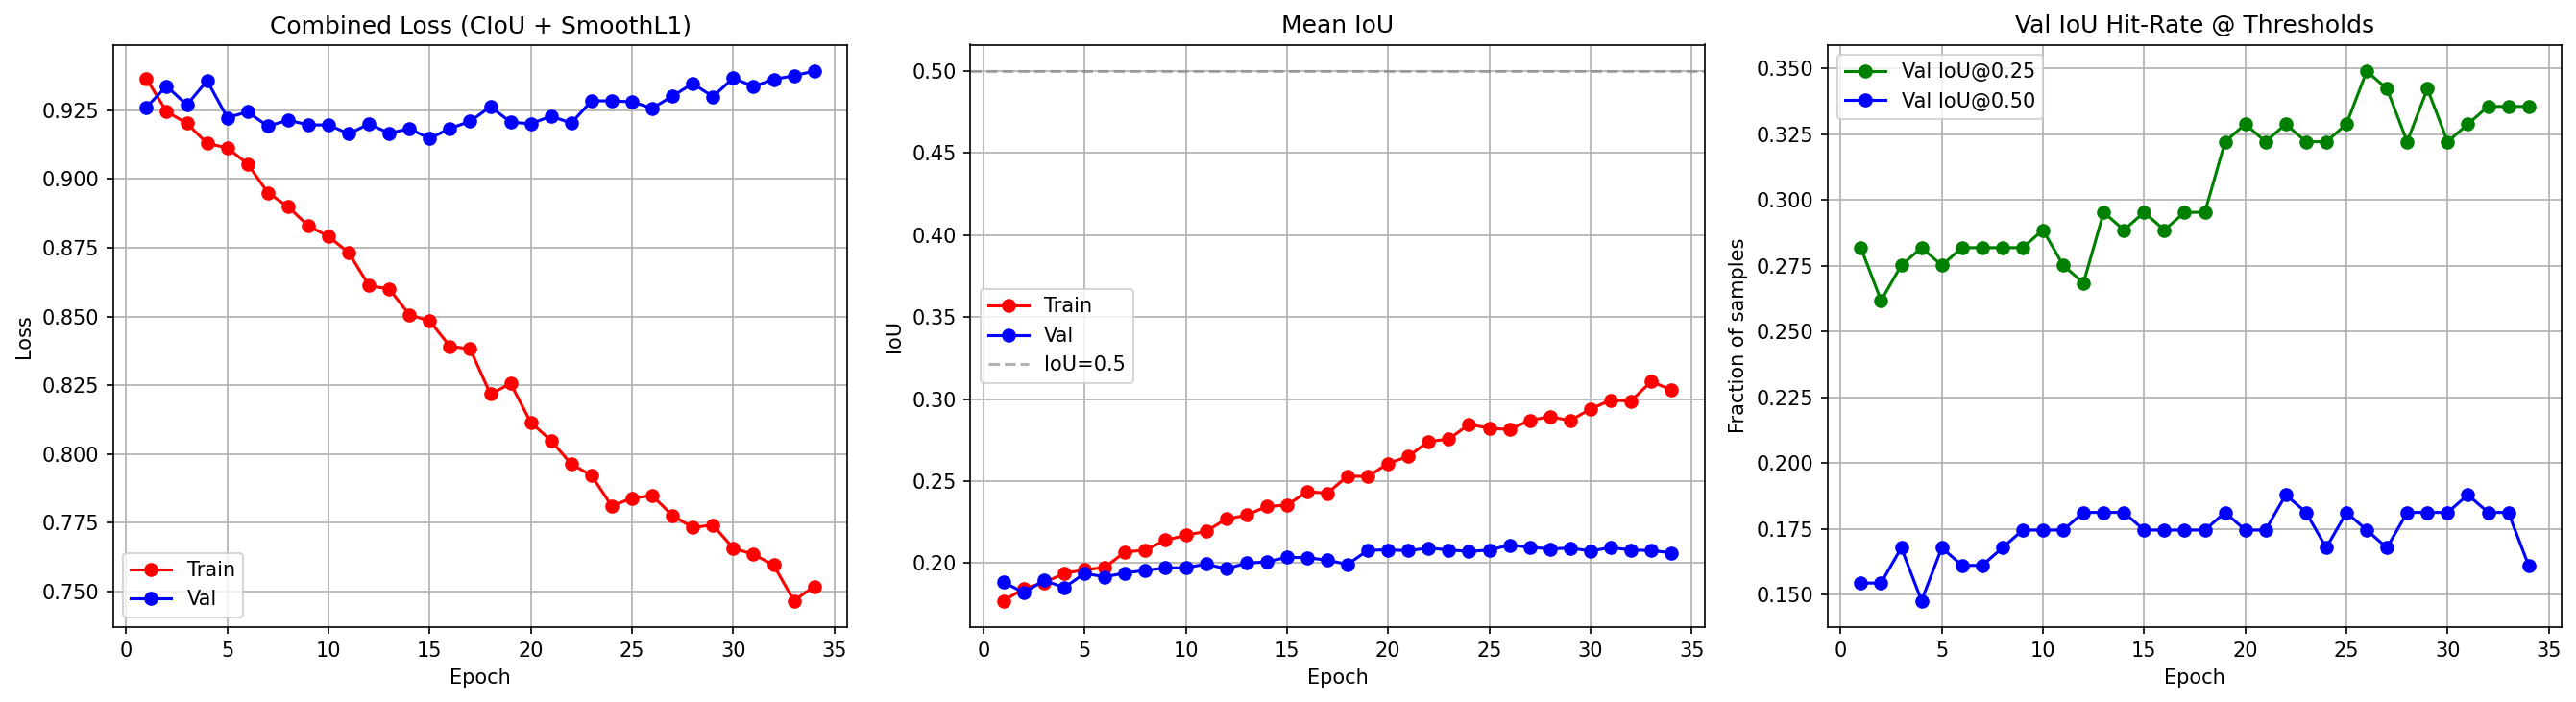
\includegraphics[width=\textwidth]{Chapter4/attachments/bbox_training_curves.png}
    \caption{Bounding box regression training curves: (left) CIoU + SmoothL1 combined loss, (centre) mean IoU, (right) validation IoU hit-rate at 0.25 and 0.50 thresholds.}
    \label{fig:bbox_curves}
\end{figure}

Per-class evaluation on the validation set reveals substantial variation across disease categories:
\FloatBarrier

\begin{table}[ht]
\centering
\caption{Per-class IoU on the bounding box validation set.}
\label{tab:bbox_perclass}
\renewcommand{\arraystretch}{1.3}
\begin{tabular}{lccc}
\toprule
\textbf{Disease} & \textbf{\#Samples} & \textbf{Mean IoU} & \textbf{IoU@0.50} \\
\midrule
Cardiomegaly   & 29  & \textbf{0.6607} & \textbf{0.828} \\
Effusion       & 31  & 0.1540          & 0.032          \\
Pneumothorax   & 20  & 0.1125          & 0.050          \\
Atelectasis    & 36  & 0.0909          & 0.000          \\
Mass           & 17  & 0.1032          & 0.000          \\
Nodule         & 16  & 0.0143          & 0.000          \\
\midrule
\textbf{Overall} & \textbf{149} & \textbf{0.2110} & \textbf{0.174} \\
\bottomrule
\end{tabular}
\end{table}

Cardiomegaly stands out with a mean IoU of 0.6607 and an IoU@0.50 hit-rate of 82.8\%, indicating near-clinical-grade localisation. This is expected: Cardiomegaly produces a large, globally positioned enlargement of the cardiac silhouette that is both structurally consistent across patients and radiologically unambiguous, making it the easiest target for a regression model. Effusion (0.154) and Pneumothorax (0.113) achieve partial localisation but fall short of the 0.5 IoU threshold for most samples. Atelectasis, Mass, and Nodule all fail to localise reliably (IoU@0.50 = 0.000), reflecting the combination of small lesion size, positional variability, and the limited annotation set of 880 samples.
\FloatBarrier
\begin{figure}[H]
    \centering
    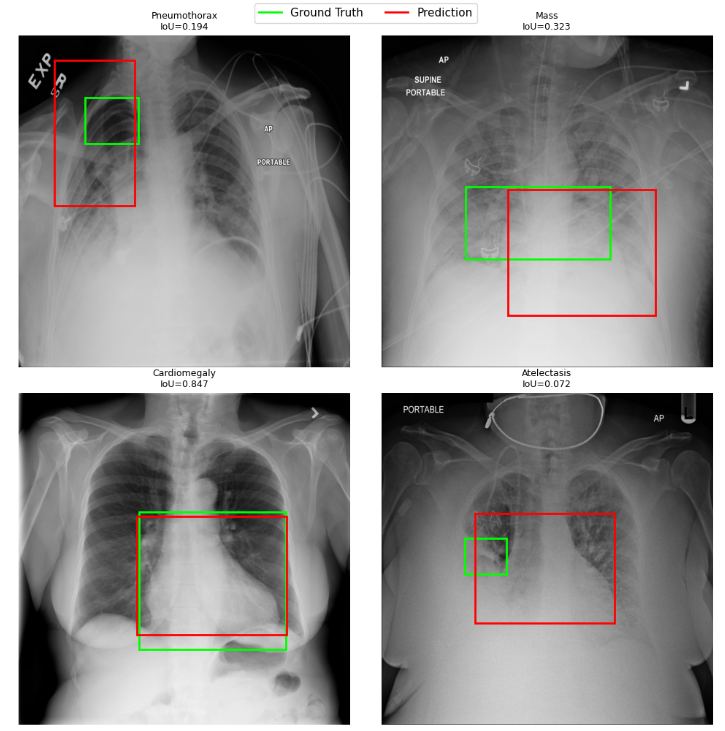
\includegraphics[
        width=\textwidth,
        height=0.5\textheight,
        keepaspectratio
    ]{Chapter4/attachments/bbox_predictions_viz.png}
    \caption{Qualitative bounding box predictions on the validation set. Green boxes denote ground-truth annotations; red boxes denote model predictions. Per-sample IoU scores are shown in the subplot titles.}
    \label{fig:bbox_viz}
\end{figure}
The overall mean IoU of 0.2110 is attributable primarily to the small size of the NIH BBox annotation set (880 samples across 8 classes). For comparison, localisation models trained on the VinBigData chest X-ray dataset, which provides radiologist-annotated bounding boxes at scale, typically achieve mean IoU in the range of \textbf{0.45--0.55}. Fine-tuning on VinBigData annotations would therefore be expected to approximately double the IoU performance.

\subsection{Lung Region Segmentation}

The Edge-Aware U-Net was trained for the full 60 epochs without early stopping. At the final epoch the model achieved:

\begin{table}[ht]
\centering
\caption{Lung segmentation performance at epoch 60 on the validation set.}
\label{tab:segmentation}
\renewcommand{\arraystretch}{1.3}
\begin{tabular}{lc}
\toprule
\textbf{Metric} & \textbf{Score} \\
\midrule
Dice Coefficient      & 0.9602 \\
IoU (Jaccard)         & 0.9249 \\
Boundary F1 (BF1)     & 0.7246 \\
Train Loss            & 0.4671 \\
Val Loss              & 0.4633 \\
\bottomrule
\end{tabular}
\end{table}
\FloatBarrier
\begin{figure}[ht]
    \centering
    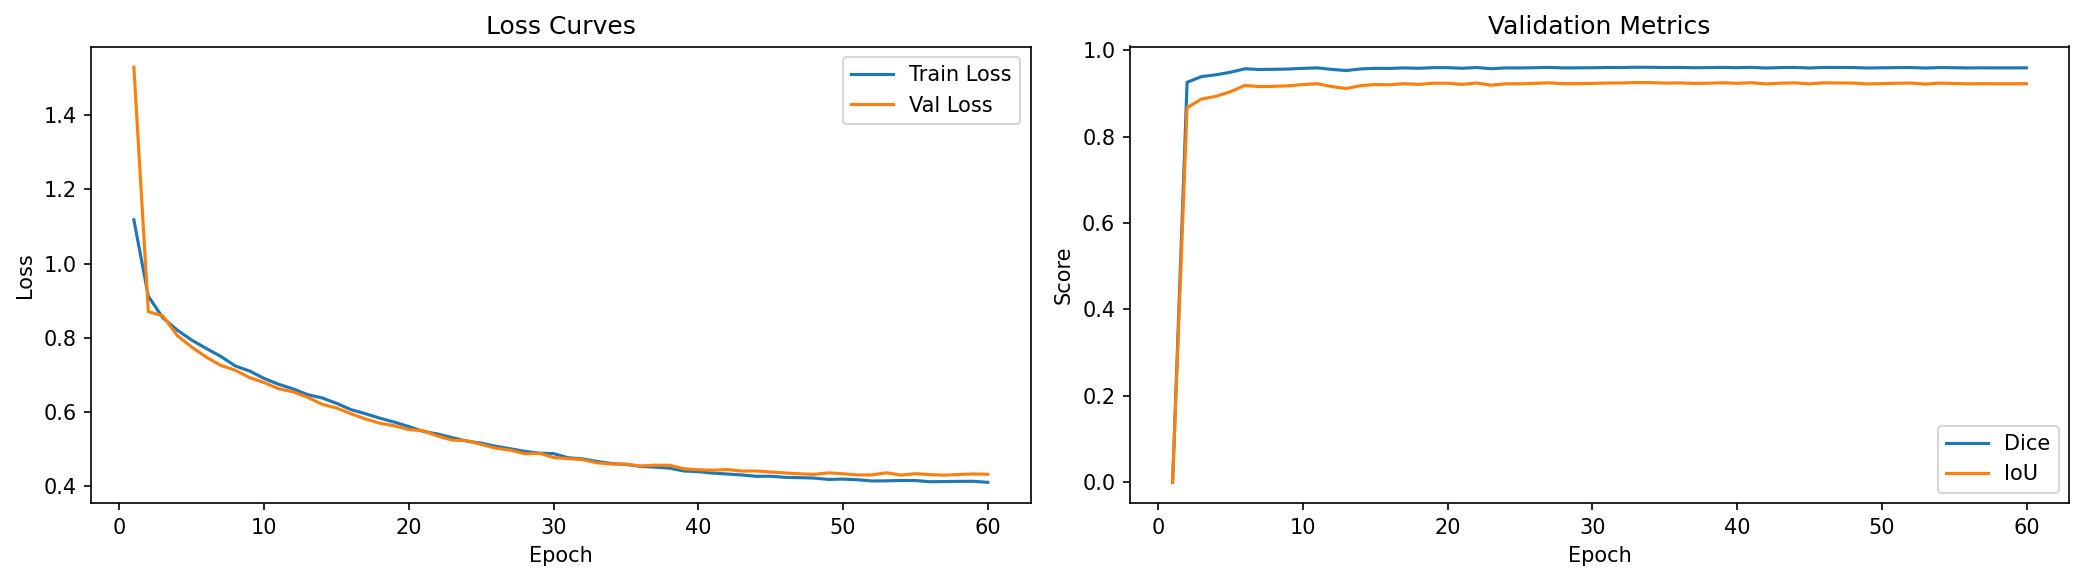
\includegraphics[width=\textwidth]{Chapter4/attachments/training_curves.png}
    \caption{Segmentation training curves: combined loss curve (train and validation) and validation metrics (Dice, IoU, Boundary F1) over 60 epochs.}
    \label{fig:seg_curves}
\end{figure}

\begin{figure}[ht]
    \centering
    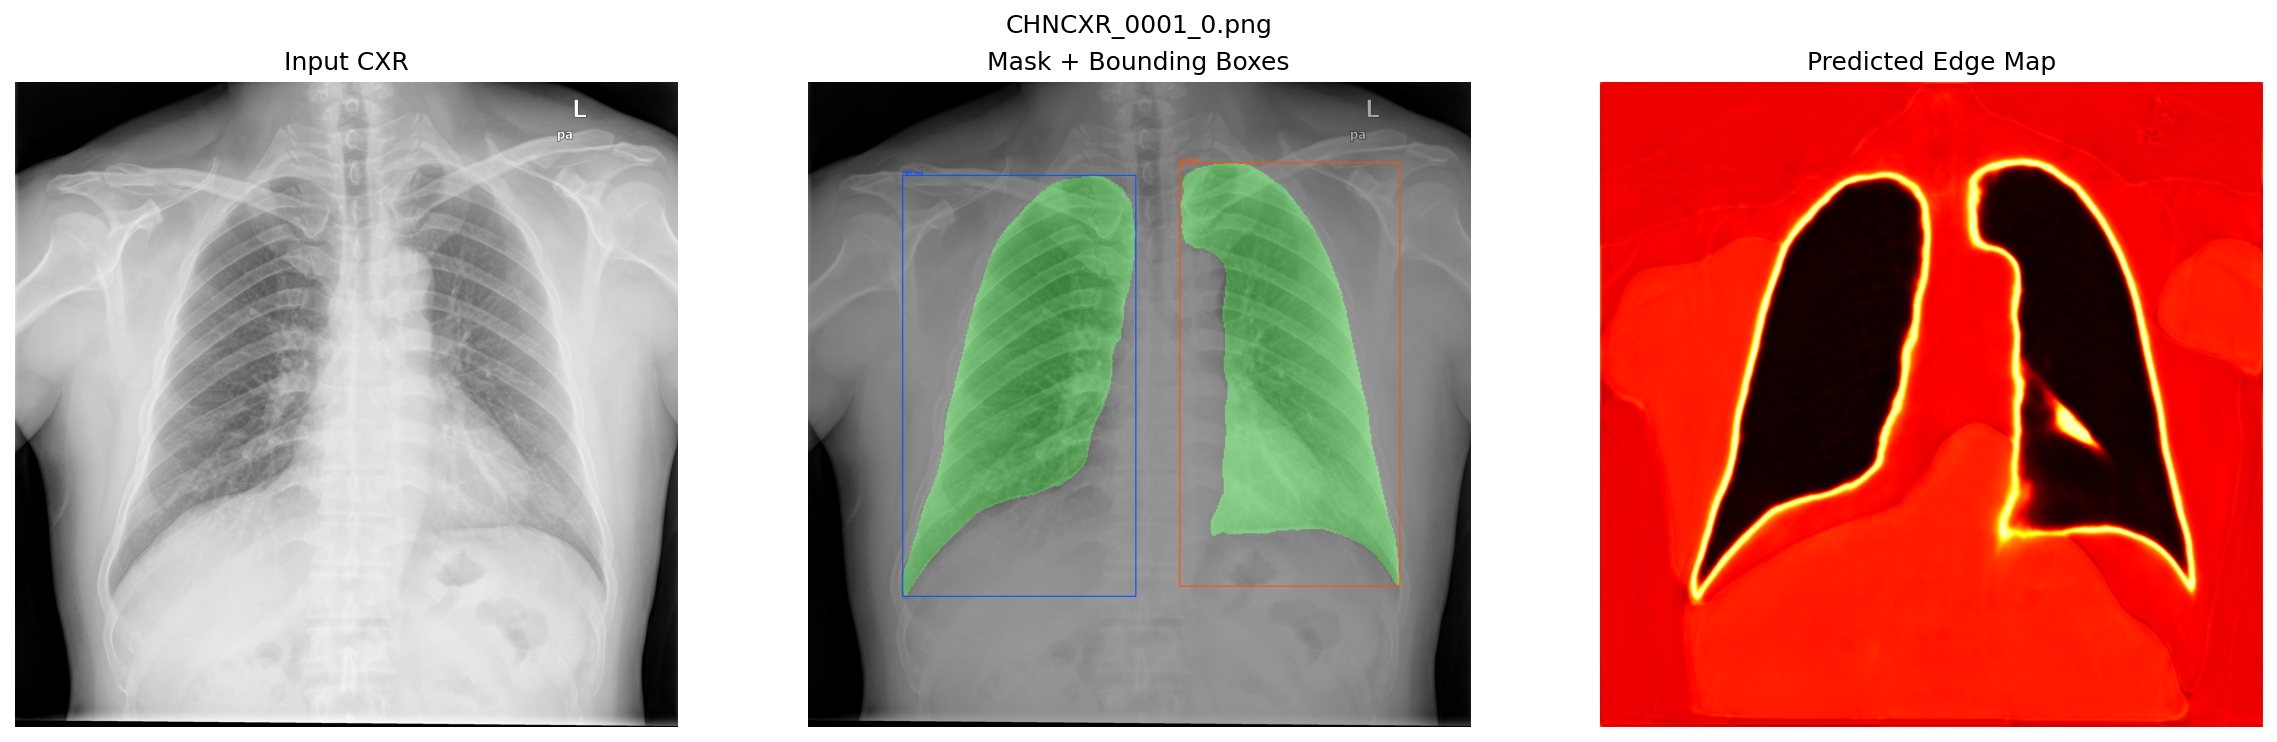
\includegraphics[width=0.75\textwidth]{Chapter4/attachments/sample_prediction.png}
    \caption{Qualitative segmentation output: predicted binary lung mask overlaid on the input radiograph with bounding boxes drawn around the segmented left and right lung fields.}
    \label{fig:seg_viz}
\end{figure}

A Dice score of \textbf{0.9589} and IoU of \textbf{0.9223} indicate near-perfect delineation of lung boundaries. The Boundary F1 of \textbf{0.7102} reflects that while overall mask overlap is excellent, fine contour precision at the lung edges particularly around the cardiac silhouette, diaphragm remains challenging. This is the region where the boundary-weighted BCE and edge head supervision provide the most benefit, and the BF1 score is expected to improve further with a larger segmentation training corpus. These segmentation outputs directly feed the zone division pipeline used for structured report generation: the left and right lung bounding boxes are subdivided into upper, middle, and lower zones, enabling zone-level disease attribution in the final radiology report.

% ------------------------------------------------------------------
\section{Summary}
\label{sec:results_summary}
% ------------------------------------------------------------------

Table~\ref{tab:results_summary} consolidates the key quantitative results across all evaluated tasks.

\begin{table}[ht]
\centering
\caption{Summary of results across all tasks.}
\label{tab:results_summary}
\renewcommand{\arraystretch}{1.3}
\begin{tabular}{llc}
\toprule
\textbf{Task} & \textbf{Metric} & \textbf{Value} \\
\midrule
SSL Pretraining              & Final SSL Loss (epoch 3)              & 0.2672 \\
Classification               & Mean AUC-ROC (13 classes)             & 0.8636 \\
Classification               & Macro F1 (default threshold)          & 0.3444 \\
Classification               & Macro F1 (optimised threshold)        & 0.5103 \\
Classification               & Micro F1 (optimised threshold)        & 0.5258 \\
Label Efficiency (50\%)      & SL+SSL AUC vs.\ SL@100\%             & 0.8608 vs.\ $\sim$0.860 \\
Label Efficiency (25\%)      & SL+SSL AUC vs.\ SL@25\%              & 0.8271 vs.\ $\sim$0.850 \\
Localisation (NIH BBox)      & Mean IoU                              & 0.2110 \\
Localisation (Cardiomegaly)  & Mean IoU / IoU@0.50                   & 0.6607 / 0.828 \\
Localisation (expected w/ VinBigData) & Mean IoU                     & $\sim$0.50 \\
Lung Segmentation            & Dice Coefficient                      & 0.9602 \\
Lung Segmentation            & IoU                                   & 0.9249 \\
Lung Segmentation            & Boundary F1                           & 0.7246 \\
\bottomrule
\end{tabular}
\end{table}

The results demonstrate that the self-supervised pretraining pipeline produces representations that generalise well across classification, localisation, and segmentation tasks. The primary classification objective achieves a mean AUC of 0.8636, outperforming all supervised-only CNN based baselines on the same dataset. The label efficiency analysis reveals that SL+SSL at 50\% of labelled data matches full-data supervised performance, confirming a meaningful reduction in annotation requirements. Threshold optimisation substantially recovers F1 performance for rare classes. Auxiliary results confirm the spatial quality of the learned features, with lung segmentation approaching near-perfect accuracy and localisation performance constrained by the limited annotation set rather than the representation quality.
% ================================================================
% Chapter 5: Conclusion and Future Scope
% Included via \input{chapter5_conclusion} in main.tex
% ================================================================

\chapter{Conclusion and Future Scope}
\label{chap:conclusion}

% ------------------------------------------------------------------
\section{Conclusion}
\label{sec:conclusion}
% ------------------------------------------------------------------

This work presented a OPTiML-inspired self-supervised pretraining pipeline for multi-label chest X-ray classification on the NIH ChestX-ray14 dataset. The SSL stage used a dense EfficientNet-B3 backbone trained with a composite loss combining optimal transport alignment, variance and covariance regularisation.

The pretrained backbone was then fine-tuned in a multimodal setup, fusing image features with patient metadata. The model achieved a mean AUC-ROC of \textbf{0.8636}, outperforming supervised-only baselines including DenseNet-121 (0.77), ViT/Swin (0.80) and EfficientNet-B3 without SSL (0.85). Strong per-class performance was seen for Emphysema (0.9714), Edema (0.9632) and Fibrosis (0.9403), while diffuse findings like Infiltration (0.7011) and Nodule (0.7538) remained more challenging due to visual ambiguity and label noise.

Threshold optimisation was an important post-processing step, improving Macro F1 from 0.3444 to \textbf{0.5103} by lowering the per-class decision boundary to a mean of 0.393. Classes like Fibrosis and Pneumonia which were completely suppressed at the default threshold of 0.5 became detectable after calibration. Auxiliary tasks further validated the spatial quality of the representations, with lung segmentation achieving Dice of \textbf{0.9589} and localisation reaching a mean IoU of 0.2110 under the limited NIH bounding box annotations, with Cardiomegaly localised at near-clinical quality (IoU = 0.6607, IoU@0.50 = 82.8\%).

The label efficiency analysis showed that SL+SSL trained on 50\% of labelled data matches full-data supervised performance, which is the most practically significant result of this work. However, at 50\% and below, the SSL-pretrained model degrades sharply, suggesting that the patch-level optimal transport objective over-specifies the representation for structural alignment at the cost of fine-grained class discriminability when labels are very scarce. Overall, OPTiML-inspired SSL pretraining shows clear promise for medical image analysis, but stabilising its performance in the low-label regime remains an open challenge that motivates the directions outlined below.

% ------------------------------------------------------------------
\section{Future Scope}
\label{sec:future}
% ------------------------------------------------------------------

\subsection{Stabilising SSL in the Low-Label Regime}

The most immediate open problem is the degradation of SL+SSL relative to SL at label fractions below 50\%. Future work should investigate modifications to the SSL objective that bring the pretraining task distribution closer to the downstream classification task, for example by incorporating pseudo-label consistency regularisation during fine-tuning, or by extending the pretraining schedule so that the optimal transport alignment has more epochs to produce representations that generalise to class boundaries rather than only structural anatomy. Curriculum-based fine-tuning, where the model is first trained on high-confidence easy samples and gradually exposed to rare classes, may also help bridge the gap.

\subsection{Localisation with VinBigData Annotations}

The current localisation module is constrained by the small NIH BBox annotation set (880 samples). Fine-tuning the bounding box regressor on the VinBigData chest X-ray dataset, which provides large-scale radiologist-annotated boxes across 14 pathology categories, is expected to raise mean IoU from the current 0.2110 to approximately 0.45--0.55. This is a straightforward extension that would make the localisation component clinically useful without any architectural changes.

\subsection{Expanding Pretraining to Larger Corpora}

The SSL backbone was pretrained exclusively on NIH ChestX-ray14. Expanding pretraining to include CheXpert, MIMIC-CXR, or PadChest would expose the backbone to substantially more diverse radiographic conditions, patient demographics, and acquisition protocols at no annotation cost. A larger and more diverse pretraining corpus is likely to improve generalisation particularly for rare pathologies and edge-case presentations, and could also close the performance gap observed at low label fractions.

\subsection{Stronger Backbones and SSL Objectives}

Applying the OPTiML objective to a Swin Transformer backbone is a natural architectural extension, given that its hierarchical attention mechanism may align more naturally with the patch-level optimal transport used in the SSL stage. On the objective side, replacing the Sinkhorn OT alignment with a masked image modelling objective such as MAE or BEiT, or combining both, could produce representations that are simultaneously spatially consistent and semantically discriminative, addressing the tension observed between structural pretraining and class-level fine-tuning at low data.

\subsection{Free-Form Report Generation}

The current report generation stage is template-driven and does not produce free-form clinical prose. Integrating a vision-language model fine-tuned on MIMIC-CXR radiology reports as a report drafting head would allow the pipeline to generate radiologist-style findings and impressions conditioned on the detected diseases, their zones, and the segmentation outputs. Replacing the horizontal zone division with lobe-aware segmentation would further improve the anatomical precision of zone-to-disease attribution in the generated reports.

%%%%%%%%%%%%%%%%%%%%%%%%%%%%%%%%%%%%%%%%%%%%%%%%%%%%
% Appendices.
% Comment out if not needed
\appendix

%%%%%%%%%%%%%%%%%%%%%%%%%%%%%%%%%%%%%%%%%%%%%%%%%%%%%%%%%%%%
% Bibliography.

\begin{singlespace}
  \bibliography{References}
  \addcontentsline{toc}{chapter}{REFERENCES}
\end{singlespace}


\end{document}
